\documentclass[11pt,a4paper]{article}

% ============================================================================
% RUET CSE 4000 -- Thesis Progress Report (2021 Series)
% Conforms strictly to Thesis_Progress_Report_Template_2021-2022.docx
% ============================================================================
\usepackage[a4paper,top=1in,bottom=1in,left=1in,right=1in]{geometry}
\usepackage[T1]{fontenc}
\usepackage[utf8]{inputenc}
\usepackage{mathptmx} % Academic serif matching Microsoft Word Times New Roman
\usepackage{amsmath,amssymb}
\usepackage{graphicx}
\usepackage{booktabs}
\usepackage{longtable}
\usepackage{tabularx}
\usepackage{multirow}
\usepackage{array}
\usepackage{xcolor}
\usepackage{colortbl}
\usepackage{float}
\usepackage{caption}
\usepackage{subcaption}
\usepackage{enumitem}
\usepackage{setspace}
\usepackage{fancyhdr}
\usepackage{titlesec}
\usepackage{tikz}
\usetikzlibrary{arrows.meta,positioning,shapes.geometric,fit,backgrounds}
\usepackage{microtype}
\usepackage[hypertexnames=false,hidelinks]{hyperref}
\setlength{\emergencystretch}{2em}

\definecolor{ruetblue}{RGB}{22,58,108}
\definecolor{ruetgray}{RGB}{242,245,249}

\onehalfspacing
\setlength{\parskip}{5.5pt}
\setlength{\parindent}{0pt}

% Headers & Footers
\pagestyle{fancy}
\fancyhf{}
\fancyhead[L]{\small\color{gray} CSE 4000 Thesis Progress Report (2021 Series)}
\fancyhead[R]{\small\color{gray} Dept.\ of CSE, RUET}
\fancyfoot[C]{\small\thepage}
\renewcommand{\headrulewidth}{0.4pt}
\renewcommand{\footrulewidth}{0.0pt}

\titleformat{\section}{\Large\bfseries\color{ruetblue}}{\thesection.}{0.6em}{}
\titleformat{\subsection}{\large\bfseries\color{ruetblue!85!black}}{\thesubsection}{0.5em}{}
\titleformat{\subsubsection}{\normalsize\bfseries}{\thesubsubsection}{0.5em}{}

\captionsetup{font=small,labelfont=bf}
\newcommand{\checkedbox}{$\boxtimes$}

\begin{document}

% ============================================================================
% OFFICIAL RUET COVER PAGE
% ============================================================================
\begin{titlepage}
\thispagestyle{empty}
\begin{center}
    {\fontsize{15}{18}\selectfont\bfseries RAJSHAHI UNIVERSITY OF ENGINEERING \& TECHNOLOGY\par}
    \vspace{4pt}
    {\fontsize{16}{19}\selectfont\bfseries Department of Computer Science \& Engineering\par}
    \vspace{16pt}
    
\includegraphics[width=2.6cm]{latex_assets/ruet_logo.png}\par
    \vspace{18pt}
    {\fontsize{16}{20}\selectfont\bfseries THESIS PROGRESS REPORT\par}
    \vspace{6pt}
    {\large\bfseries CSE 4000 -- Thesis/Project\par}
    {\large 4th Year Even Semester \quad|\quad 2021 Series\par}
    \vspace{18pt}
    \rule{\textwidth}{1.0pt}\par
    \vspace{10pt}
    {\fontsize{15}{20}\selectfont\bfseries Title:\par}
    \vspace{4pt}
    {\fontsize{13.5}{18}\selectfont\bfseries Spaceborne SAR Ship Wake Analysis for Vessel Maneuver Recognition Using Hydrodynamic Wake Geometry, Hybrid scSE-Radon Segmentation, and Dual-Scale Deep Vision Ensembles\par}
    \vspace{10pt}
    \rule{\textwidth}{1.0pt}\par
\end{center}

\vspace{16pt}
\noindent
\begin{minipage}[t]{0.53\textwidth}
    {\large\bfseries Submitted By}\par
    \vspace{8pt}
    \textbf{Student 1:}\par
    \textbf{Name:} Md.\ Wariul Mohaimin\par
    \textbf{Roll No.:} 2103001\par
    \textbf{Registration No.:} 544\par
    \vspace{8pt}
    \textbf{Student 2:}\par
    \textbf{Name:} Md.\ Mostain Billa Rifat\par
    \textbf{Roll No.:} 2103023\par
    \textbf{Registration No.:} 566\par
    \vspace{10pt}
    \textbf{Session:} 2021--2022\par
    \textbf{Year--Semester:} 4th Year Even Semester\par
    Department of Computer Science \& Engineering\par
    Rajshahi University of Engineering \& Technology\par
    Rajshahi-6204, Bangladesh
\end{minipage}%
\hfill
\begin{minipage}[t]{0.43\textwidth}
    {\large\bfseries Supervised By}\par
    \vspace{8pt}
    \textbf{Name:} Dr.\ Julia Rahman\par
    \textbf{Designation:} Associate Professor\par
    Department of Computer Science \& Engineering\par
    Rajshahi University of Engineering \& Technology (RUET)\par
    Rajshahi-6204, Bangladesh
\end{minipage}

\vfill
\begin{center}
    {\small\color{gray} Report Submission Date: November 28, 2026}
\end{center}
\end{titlepage}

% ============================================================================
% FRONT MATTER: METADATA SUMMARY TABLE + TOC
% ============================================================================
\pagenumbering{roman}
\section*{Progress Report Overview}
\addcontentsline{toc}{section}{Progress Report Overview}

Table~\ref{tab:overview} summarizes the administrative, computational, and dataset profile of our thesis work in exact alignment with the Department of CSE, RUET Thesis Progress Report template (\texttt{CSE 4000}).

\begin{table}[H]
\centering
\caption{Thesis Progress Report Administrative and Technical Summary}
\label{tab:overview}
\begin{tabularx}{\textwidth}{|l|X|}
\hline
\rowcolor{ruetgray}
\textbf{Item} & \textbf{Description} \\ \hline
Course Code & CSE 4000 \\ \hline
Course Title & Thesis/Project \\ \hline
Series & 2021 (Session: 2021--2022) \\ \hline
Semester & 4th Year Even Semester \\ \hline
Thesis Duration & October 2026 -- Ongoing (4th Year Even Semester Progress Review) \\ \hline
Report Type & Progress Report \\ \hline
Area of Research & Spaceborne Remote Sensing, Computer Vision, Maritime Domain Awareness, Physics-Guided Deep Learning \\ \hline
Research Type & Applied Quantitative Empirical Research \& Multimodal Deep Learning Systems Engineering \\ \hline
Tools \& Technologies & Python 3.11, PyTorch (AMP FP16/CUDA), \texttt{timm} (\texttt{ConvNeXt-Tiny}, \texttt{SwinV2-Tiny}), \texttt{segmentation-models-pytorch} (ResNet-50 U-Net + scSE), Scikit-Image (Radon Transform, Skeletonization), OpenCV (CLAHE, Lee Speckle Filter), Scikit-Learn (HistGradientBoosting), Kaggle P100/T4 Cloud GPUs, Git \\ \hline
Dataset Source & 100\% Authentic Sentinel-1 IW GRD Imagery paired with Synchronous AIS Telemetry: \textbf{UEIKAP\_DATASET} (Zenodo DOI: 10.5281/zenodo.18391027) and \textbf{MMDEC} (Zenodo DOI: 10.5281/zenodo.17491518) \\ \hline
\end{tabularx}
\end{table}

\tableofcontents
\newpage
\listoffigures
\listoftables
\newpage

\pagenumbering{arabic}
\setcounter{page}{1}

% ============================================================================
% SECTION 1: THESIS IN BRIEF
% ============================================================================
\section{Thesis in Brief}

Modern maritime domain awareness relies heavily on the Automatic Identification System (AIS), a cooperative VHF radio broadcast mandated for commercial vessels. However, non-compliant actors---including illegal, unreported, and unregulated (IUU) fishing trawlers, sanction-evading tankers conducting ship-to-ship oil transfers, and coastal smugglers---frequently switch off or spoof their AIS transponders, turning into ``dark vessels.'' Spaceborne Synthetic Aperture Radar (SAR), exemplified by the European Space Agency's (ESA) Sentinel-1 C-band constellation ($5.405$\,GHz), defeats radio evasion because active microwave pulses image the ocean surface reliably at night and through dense cloud cover. Even when a ship hull is small or barely separable from sea clutter in 10\,m imagery, its displacement creates hydrodynamic surface waves stretching several kilometers astern. Whether that wake runs symmetrically straight or curves asymmetrically reveals directly whether the vessel is cruising steadily or executing a turning maneuver.

In this thesis, we develop and rigorously validate a ``Zero-AIS at Inference'' radar computer vision pipeline that predicts vessel maneuver states (\textit{Straight} vs.\ \textit{Turning}), auxiliary chirality (\textit{Port} vs.\ \textit{Starboard}), continuous rate of turn (ROT), and epistemic prediction uncertainty solely from satellite SAR scenes. Over seven iterative engineering eras between October and November 2026, our team systematically dismantled real-world physical bottlenecks: we recovered submerged wake signals from dark ocean pixels ($2.5$\,DN mean lifted to $75.3$\,DN), integrated U-Net segmentation (\textit{Wake-Net} with scSE attention) and Radon/PCA curvature descriptors, expanded from 449 UEIKAP vessels to \textbf{4,108 strictly trajectory-verified ships} across UEIKAP and MMDEC, caught and removed a subtle AIS sensor-byte corruption trap, and verified a D4 chirally symmetric \texttt{ConvNeXt-Tiny} + \texttt{SwinV2-Tiny} dual-scale ensemble attaining \textbf{0.8165 combined ROC-AUC} (\textbf{0.8334 on MMDEC}, \textbf{0.8572 on clear tactical turns} $|\text{ROT}|\ge 2.0^\circ$/min, and \textbf{0.9001 AUC} under Monte Carlo Dropout analyst triage) with \textbf{zero overfitting}.

% ============================================================================
% SECTION 2: ABSTRACT
% ============================================================================
\section{Abstract}

Detecting active vessel maneuvers solely from spaceborne Synthetic Aperture Radar (SAR) imagery without Automatic Identification System (AIS) broadcasts at inference time is a critical capability for maritime surveillance, yet remains challenging due to specular microwave darkness over calm seawater, multiplicative Rayleigh speckle noise, scarcity of maneuvering examples, and noisy shipborne telemetry. This progress report documents the complete mathematical formulation, software engineering evolution, forensic bug discovery, and experimental validation of a physics-guided multimodal deep learning framework trained strictly on authentic Sentinel-1 Interferometric Wide Swath (IW) Ground Range Detected (GRD) acquisitions.

First, to counteract severe dynamic-range compression in raw Sentinel-1 GRD products---where over 99\% of open-ocean pixels lie at or below 5 digital numbers (DN)---we introduce a domain-consistent luminance normalizer paired with percentile range stretching ($P_{1.0}$--$P_{99.5}$), Contrast Limited Adaptive Histogram Equalization (CLAHE), and adaptive $7\times 7$ Lee speckle filtering. Second, we train a 3-channel Hybrid \textit{Wake-Net} (ResNet-50 U-Net enhanced with spatial and channel Squeeze-and-Excitation attention), adapted to open-water sea states via train-only pseudo-labeling and morphological hysteresis masking, from which sparse Radon transforms and linear-versus-quadratic Principal Component Analysis (PCA) curve fits extract 20 interpretable hydrodynamic geometry descriptors. Third, to break both the low-data bottleneck in UEIKAP ($N_{\text{turn}}=76$ training ships) and the $0.27$-pixel Sentinel-1 spatial Nyquist observability bound, we scale to the Multimodal Maritime Dataset on the English Channel (MMDEC) using unwrapped multi-ping $d(\text{COG})/dt$ trajectory fitting across 19 million AIS records while permanently eliminating corrupted onboard \texttt{RateOfTurn} sensor fallbacks whose turning precision measured only 19.4\%.

Across 594 unseen, MMSI-disjoint test vessels drawn from 4,108 verified ships (2,886 Straight and 1,222 Turning), a D4 chirally equivariant Dual-Scale \texttt{ConvNeXt-Tiny} + \texttt{SwinV2-Tiny} + Geometry MLP ensemble reaches \textbf{0.8165 combined ROC-AUC}, \textbf{0.6937 PR-AUC}, \textbf{76.10\% Straight accuracy}, and \textbf{72.39\% Turning accuracy} at default cutoff $\tau=0.52$ (\textbf{79.35\% Straight} / \textbf{69.94\% Turning} at $\tau=0.56$), while reaching \textbf{0.8334 ROC-AUC} (\textbf{77.12\% Straight}, \textbf{74.83\% Turning}) on pure MMDEC encounters and \textbf{0.8572 ROC-AUC} (\textbf{78.72\% Turning}) on clear tactical turns ($|\text{ROT}|\ge 2.0^\circ$/min). Audited Train--Validation AUC gaps remain essentially zero ($-0.0072$ for \texttt{ConvNeXt-Tiny} and $+0.0259$ for \texttt{SwinV2-Tiny}), and 30-pass Monte Carlo Dropout triage improves confident-subset discrimination to \textbf{0.8918--0.9001 ROC-AUC} (\textbf{84.85\%--86.92\% overall accuracy}).

% ============================================================================
% SECTION 3: OBJECTIVES OF THE THESIS
% ============================================================================
\section{Objectives of the Thesis}

\subsection{Main Objectives}
\begin{enumerate}[label=\roman*),leftmargin=2em]
    \item \textbf{Zero-AIS Operational Deployment:} Build an inference pipeline capable of distinguishing straight cruising vessels from actively maneuvering vessels exclusively from spaceborne Sentinel-1 SAR scenes without consuming AIS telemetry at prediction time.
    \item \textbf{Radar Dynamic-Range and Speckle Recovery:} Design radar-tailored contrast stretching, polarimetric luminance unification, and Lee speckle denoising to preserve weak $1$--$3$\,DN Kelvin wake ridges and turbulent centerline tracks against sea clutter.
    \item \textbf{Physics-Guided Multimodal Representation:} Couple deep segmentation (\textit{Wake-Net} scSE masks) and analytical wake descriptors (Radon angular variance, centerline curvature, and quadratic PCA bend) with modern dual-scale visual backbones (\texttt{ConvNeXt-Tiny} and \texttt{SwinV2-Tiny}).
    \item \textbf{Authentic Large-Scale Zero-Leakage Benchmarking:} Strictly prohibit synthetic/GAN SAR imagery, resolve AIS telemetry labeling corruption via unwrapped multi-ping course trajectories, and enforce MMSI-disjoint partitioning across UEIKAP and MMDEC.
    \item \textbf{Verifiable Generalization, Explainability, and Operational Triage:} Prove absence of overfitting via live Train--Validation AUC gap auditing, validate causal reliance on wakes through counterfactual erasures and feature permutation, and integrate Monte Carlo Dropout uncertainty rejection for analyst decision support.
\end{enumerate}

\subsection{Specific Research Questions}
\begin{enumerate}[label=\roman*),leftmargin=2em]
    \item \textbf{RQ1 (Dynamic Range Compression):} How severely does specular microwave darkening over calm ocean waters degrade standard deep CNNs, and what gain does percentile contrast recovery paired with CLAHE and Lee filtering provide?
    \item \textbf{RQ2 (Spatial Nyquist Resolution Floor):} How do vessel speed, angular Rate of Turn (ROT), and Sentinel-1's 10\,m ground sampling distance interact to impose a physical detection limit on mild trajectory corrections?
    \item \textbf{RQ3 (Trajectory Derivative vs.\ Sensor Fallback):} Can uncalibrated shipborne \texttt{RateOfTurn} AIS sensor bytes distort supervised maneuver training compared to unwrapped multi-ping $d(\text{COG})/dt$ kinematic regression?
    \item \textbf{RQ4 (Chiral Symmetry \& Dual-Scale Fusion):} Does aligning wake axes across macro and stern-zoomed views under exact $D_4$ dihedral equivariance improve turning recall without overfitting to vessel heading or background wave orientation?
    \item \textbf{RQ5 (Human-in-the-Loop Safety):} Can predictive entropy from stochastic Monte Carlo Dropout forward passes reliably flag high-risk false alarms and sea-clutter ambiguities for deferred analyst review?
\end{enumerate}

% ============================================================================
% SECTION 4: LITERATURE REVIEW STATUS
% ============================================================================
\section{Literature Review Status}

To place our architecture within current remote sensing and maritime computer vision research, we reviewed primary archival literature spanning radar hydrodynamics, deep wake segmentation, maritime benchmarks, and trustworthy machine learning:

\begin{itemize}[leftmargin=1.5em]
    \item \textbf{Number of papers and datasets reviewed:} 10 core foundational works (8 peer-reviewed papers and doctoral theses plus 2 large-scale open Sentinel-1/AIS benchmarks).
    \item \textbf{Indexed journals and conferences covered:} IEEE Transactions on Geoscience and Remote Sensing (TGRS), IEEE Geoscience and Remote Sensing Letters (GRSL), Proceedings of SPIE Remote Sensing, CVPR, ICCV, ICML, DLR / Helmut-Schmidt-Universit\"at Monograph, and Virginia Tech PhD Dissertation.
    \item \textbf{Key methodologies identified:} Localized Radon transform wake peak detection~\cite{graziano2016ship}; empirical wind/speed SAR wake visibility characterization~\cite{tings2024erkennung}; U-Net with scSE attention for fragmented radar wakes~\cite{zhang2023wakenet}; contextual EO/SAR meteo-marine fusion~\cite{mazzeo2024spie_ueikap}; oriented wake box detection~\cite{xu2024opensarwake}; hierarchical depthwise CNNs~\cite{liu2022convnext}; Grad-CAM localization~\cite{selvaraj2017gradcam}; and Bayesian MC-Dropout uncertainty~\cite{gal2016dropout}.
    \item \textbf{Research gap identified:} Prior radar wake systems predominantly model \textit{straight} ship tracks for speed and heading recovery~\cite{graziano2016ship}, focus strictly on wake bounding-box or mask detection~\cite{zhang2023wakenet,xu2024opensarwake}, or rely on small/simulated datasets~\cite{mazzeo2026ueikap,higgins2023machine}. Large-scale empirical validation of active \textit{turning maneuver detection} across thousands of trajectory-verified real Sentinel-1 encounters---together with sensor-noise forensics and zero-overfit guarantees---remained largely unexplored.
\end{itemize}

\subsection{Summary of Reviewed Papers}

A concise technical synthesis of each primary reference follows before Table~\ref{tab:lit_summary}:

\begin{itemize}[leftmargin=1.5em]
    \item \textbf{Graziano, D'Errico, \& Rufino (IEEE TGRS, 2016)~\cite{graziano2016ship}:} Pioneered localized Radon transform integration inside annular windows around detected SAR ship hulls, resolving ship heading ($\pm 1^\circ$--$3^\circ$) and velocity from divergent Kelvin wave arms. While mathematically elegant for steady cruising, its linear Radon integral breaks down when a turning rudder bends the centerline wake along a circular arc.
    \item \textbf{Tings (Helmut-Schmidt-Univ.\ / DLR, 2024)~\cite{tings2024erkennung}:} Established comprehensive physical detectability envelopes for Kelvin and turbulent wakes across C-band and X-band SAR under varying wind speed, incidence angles, and ship dimensions. This work anchors our failure taxonomy around low-Froude-number calm seas and gale-force wave clutter masking.
    \item \textbf{Zhang et al.\ (Wake-Net, IEEE TGRS, 2023)~\cite{zhang2023wakenet}:} Introduced spatial-and-channel Squeeze-and-Excitation (scSE) residual blocks into a U-Net wake segmenter to recover broken radar wake segments from heavy sea speckle. However, \textit{Wake-Net} outputs pixel masks only and performs neither maneuver state recognition nor uncertainty estimation.
    \item \textbf{Mazzeo, Graziano et al.\ (UEIKAP, SPIE 2024 \& Zenodo 2026)~\cite{mazzeo2024spie_ueikap,mazzeo2026ueikap}:} Released the first open multi-modal benchmark pairing Sentinel-1 SAR and Sentinel-2 optical chips with interpolated AIS telemetry and polygon wake ground truth (515 SAR scenes). Its thorough physical annotation inspired our early fusion baselines, though its small pool of active turning ships ($N_{\text{turn}}=104$) necessitated dataset expansion.
    \item \textbf{Xu \& Wang (OpenSARWake, IEEE GRSL, 2024)~\cite{xu2024opensarwake}:} Curated a large-scale SAR oriented bounding-box wake benchmark paired with feature-refinement detectors. While effective for wake localization, OpenSARWake lacks synchronized AIS rotational kinematics to separate gentle turns from straight navigation.
    \item \textbf{Averty, Nasios, Ray, \& Piliouras (MMDEC, Zenodo 2025)~\cite{averty_mmdec}:} Published 230 Sentinel-1 scenes across the English Channel paired with 19 million AIS pings and \texttt{SatShipAI} ship radar positions. We discovered that raw onboard \texttt{RateOfTurn} bytes inside AIS are frequently uncalibrated, requiring multi-ping $d(\text{COG})/dt$ trajectory extraction to unlock MMDEC for clean maneuver learning.
    \item \textbf{Higgins (Virginia Tech PhD Thesis, 2023)~\cite{higgins2023machine}, Liu et al.\ (CVPR, 2022)~\cite{liu2022convnext}, Selvaraju et al.\ (ICCV, 2017)~\cite{selvaraj2017gradcam}, \& Gal and Ghahramani (ICML, 2016)~\cite{gal2016dropout}:} Provided, respectively, evidence for physics-image fusion (in simulated wakes), the $7\times 7$ depthwise ConvNeXt spatial inductive bias, gradient localization auditing, and Bayesian dropout entropy for operational deferral.
\end{itemize}

{\small
\begin{longtable}{|p{2.5cm}|p{2.7cm}|p{2.1cm}|p{2.9cm}|p{2.7cm}|}
\caption{Structured Comparison Matrix of Core Literature and Benchmarks}
\label{tab:lit_summary} \\
\hline
\rowcolor{ruetgray}
\textbf{Paper / Dataset \& Year} & \textbf{System Methodology} & \textbf{Dataset} & \textbf{Contribution} & \textbf{Limitations} \\ \hline
\endfirsthead
\hline
\rowcolor{ruetgray}
\textbf{Paper / Dataset \& Year} & \textbf{System Methodology} & \textbf{Dataset} & \textbf{Contribution} & \textbf{Limitations} \\ \hline
\endhead
1.\ Graziano et al., IEEE TGRS, 2016~\cite{graziano2016ship} & Localized Radon Transform on linear Kelvin wake arms & TerraSAR-X / Sentinel-1 case study & Sub-degree straight ship heading \& speed estimation & Linear model; degrades during curved turning maneuvers \\ \hline
2.\ Tings, DLR Monograph, 2024~\cite{tings2024erkennung} & Empirical wake visibility across C/X-band sea states & Multi-sensor C- \& X-band SAR archive & Quantitative wind, Froude, and incidence detectability bounds & Does not classify maneuvering state end-to-end \\ \hline
3.\ Zhang et al.\ (Wake-Net), IEEE TGRS, 2023~\cite{zhang2023wakenet} & U-Net with scSE decoder attention & C-band SAR wake segmentation benchmark & Suppresses speckle and reconnects fragmented wake tracks & Pixel segmentation only; no kinematic maneuver head \\ \hline
4.\ Mazzeo et al.\ (UEIKAP), SPIE 2024 / Zenodo 2026~\cite{mazzeo2024spie_ueikap,mazzeo2026ueikap} & EO/SAR wake detection + sea-state context & 515 S1 SAR chips + 522 AIS CSVs & Open public SAR-AIS benchmark with polygon wake masks & Small turning sample ($N=104$); severe class imbalance \\ \hline
5.\ Xu \& Wang (OpenSARWake), IEEE GRSL, 2024~\cite{xu2024opensarwake} & Feature-refinement oriented OBB wake detector & Large-scale SAR oriented wake crops & Strong wake localization across sea states & Bounding-box task without AIS ROT maneuver ground truth \\ \hline
6.\ Averty et al.\ (MMDEC), Zenodo, 2025~\cite{averty_mmdec} & Synchronized S1 tiles + AIS + SatShipAI & 230 S1 scenes, 19M AIS pings & Large-scale English Channel radar-AIS archive & Raw AIS ROT bytes noisy; requires $d(\text{COG})/dt$ filtering \\ \hline
7.\ Higgins, Va.\ Tech PhD Thesis, 2023~\cite{higgins2023machine} & ML \& data fusion on wake descriptors & Simulated hydrodynamic wake scenes & Shows physics fusion potential for wake inference & Validated on simulated wakes rather than real spaceborne SAR \\ \hline
8.\ Liu et al.\ (ConvNeXt), CVPR, 2022~\cite{liu2022convnext} & Modernized $7\times 7$ depthwise ConvNet & ImageNet-1K & Wide receptive field rivaling vision transformers & Requires radar contrast recovery \& chiral symmetry adaptation \\ \hline
9.\ Gal \& Ghahramani, ICML, 2016~\cite{gal2016dropout} & Stochastic test-time dropout passes & Image/tabular uncertainty benchmarks & Lightweight epistemic entropy \& rejection curves & Unapplied to dark-vessel radar maneuver triage prior to us \\ \hline
10.\ Selvaraju et al.\ (Grad-CAM), ICCV, 2017~\cite{selvaraj2017gradcam} & Feature-map gradient attribution & Vision CNNs & Visual confirmation of localized object attention & Cannot replace causal wake erasure tests \\ \hline
\end{longtable}
}

\subsection{Structured Literature Analysis}
\begin{itemize}[leftmargin=1.5em]
    \item \textbf{Major Works:} Maritime radar analytics centers either on classical Radon integrals for steady trajectories~\cite{graziano2016ship} or standalone segmentation/detection networks~\cite{zhang2023wakenet,xu2024opensarwake}, while authentic maneuver recognition suffered from small dataset sizes~\cite{mazzeo2026ueikap} or simulated substitutes~\cite{higgins2023machine}.
    \item \textbf{Research Gap:} No open study addresses end-to-end Zero-AIS maneuvering inference at 4,000+ real vessel scale while uniting specular dynamic-range preprocessing, the $0.27$-pixel spatial Nyquist boundary, trajectory-verified AIS de-noising, and chiral dual-scale vision transformers with explicit overfitting control.
    \item \textbf{Proposed Work Difference:} We construct a unified 3-stage system that: (1) normalizes multi-source Sentinel-1 dynamic ranges and segments wakes via domain-adapted scSE \textit{Wake-Net}; (2) computes 20 Radon/skeleton/PCA wake curvature features; and (3) fuses global and stern-aligned wake crops across \texttt{ConvNeXt-Tiny} and \texttt{SwinV2-Tiny} under exact $D_4$ chiral symmetry, verified against a 4,108-vessel trajectory benchmark.
\end{itemize}

% ============================================================================
% SECTION 5: METHODOLOGY
% ============================================================================
\section{Methodology}

\subsection{Overview}
Our methodology bridges classical ocean wave physics and modern deep learning without allowing the deployed model any access to shipboard AIS transponders during prediction. Offline, synchronous AIS trajectories strictly label ground-truth maneuvers. Online (at test/inference time), a single raw Sentinel-1 SAR chip flows sequentially through: (1) cross-domain luminance calibration, CLAHE stretching, and $7\times 7$ Lee filtering; (2) 3-channel scSE \textit{Wake-Net} segmentation; (3) skeletonization, Radon transform, and quadratic PCA centerline fitting; and (4) a D4 chirally symmetric \texttt{DualScaleWakeNet} ensemble outputting maneuver state probabilities and Monte Carlo Dropout uncertainty scores (Figure~\ref{fig:methodology_flow}).

\begin{figure}[H]
\centering
\resizebox{0.98\textwidth}{!}{%
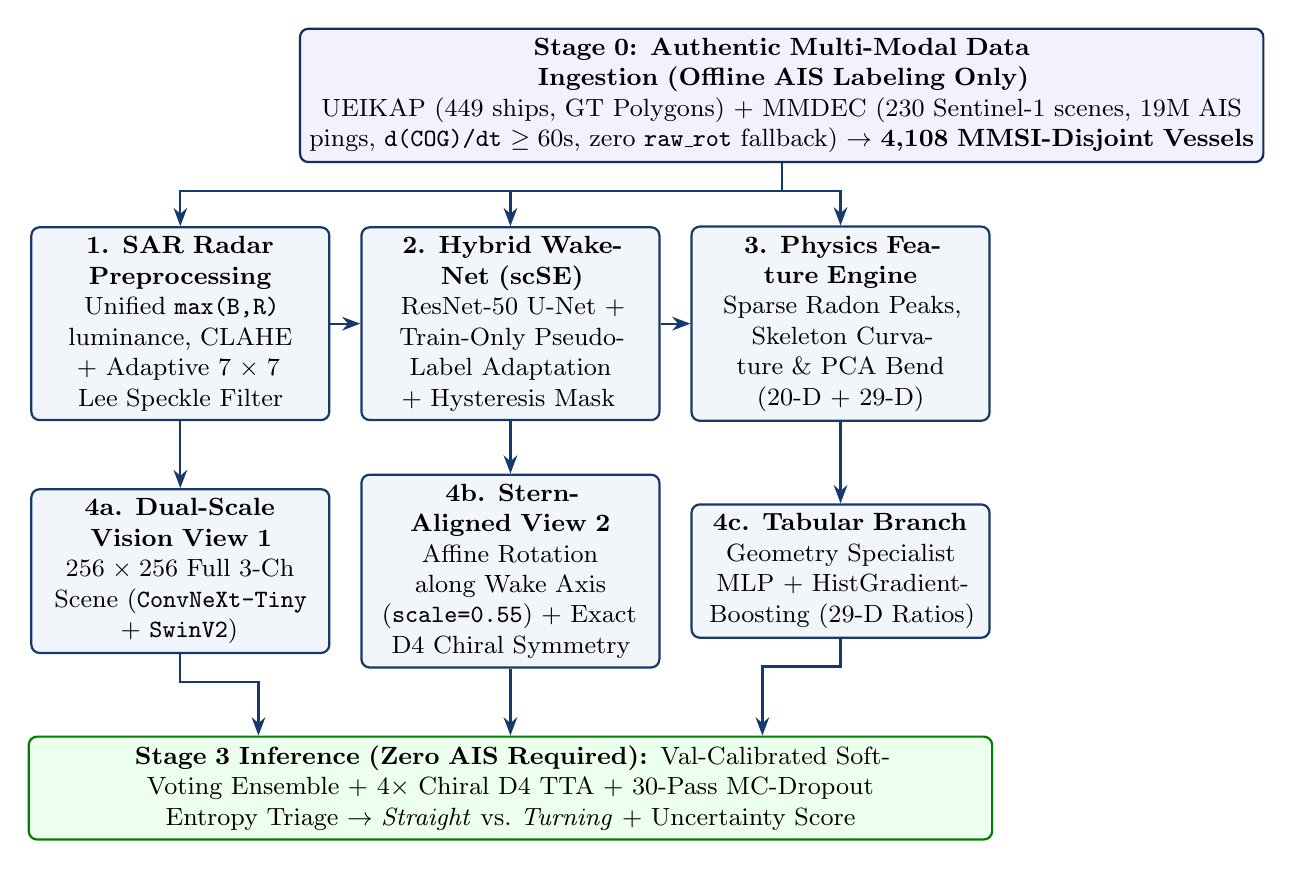
\begin{tikzpicture}[
    node distance=0.65cm and 0.7cm,
    box/.style={rectangle, draw=ruetblue, thick, fill=ruetgray, rounded corners=3pt, text width=3.55cm, align=center, minimum height=1.15cm, font=\small},
    widebox/.style={rectangle, draw=ruetblue!80!black, thick, fill=blue!5, rounded corners=3pt, text width=12.0cm, align=center, minimum height=0.95cm, font=\small},
    arrow/.style={->, >=Stealth, thick, color=ruetblue}
]
\node[widebox] (data) {\textbf{Stage 0: Authentic Multi-Modal Data Ingestion (Offline AIS Labeling Only)}\\
UEIKAP (449 ships, GT Polygons) + MMDEC (230 Sentinel-1 scenes, 19M AIS pings, \texttt{d(COG)/dt} $\ge 60$s, zero \texttt{raw\_rot} fallback) $\rightarrow$ \textbf{4,108 MMSI-Disjoint Vessels}};

\node[box, below left=0.8cm and -0.4cm of data] (prep) {\textbf{1. SAR Radar Preprocessing}\\Unified \texttt{max(B,R)} luminance, CLAHE + Adaptive $7\times 7$ Lee Speckle Filter};
\node[box, right=0.38cm of prep] (wnet) {\textbf{2. Hybrid Wake-Net (scSE)}\\ResNet-50 U-Net + Train-Only Pseudo-Label Adaptation + Hysteresis Mask};
\node[box, right=0.38cm of wnet] (geom) {\textbf{3. Physics Feature Engine}\\Sparse Radon Peaks, Skeleton Curvature \& PCA Bend (20-D + 29-D)};

\node[box, below=0.85cm of prep] (macro) {\textbf{4a. Dual-Scale Vision View 1}\\$256\times 256$ Full 3-Ch Scene (\texttt{ConvNeXt-Tiny} + \texttt{SwinV2})};
\node[box, right=0.38cm of macro] (stern) {\textbf{4b. Stern-Aligned View 2}\\Affine Rotation along Wake Axis (\texttt{scale=0.55}) + Exact D4 Chiral Symmetry};
\node[box, right=0.38cm of stern] (mlp) {\textbf{4c. Tabular Branch}\\Geometry Specialist MLP + HistGradientBoosting (29-D Ratios)};

\node[widebox, below=0.85cm of stern, fill=green!7, draw=green!50!black] (out) {\textbf{Stage 3 Inference (Zero AIS Required):} Val-Calibrated Soft-Voting Ensemble + $4\times$ Chiral D4 TTA + 30-Pass MC-Dropout Entropy Triage $\rightarrow$ \textit{Straight} vs.\ \textit{Turning} + Uncertainty Score};

\draw[arrow] (data.south) -- ++(0,-0.35) -| (prep.north);
\draw[arrow] (data.south) -- ++(0,-0.35) -| (wnet.north);
\draw[arrow] (data.south) -- ++(0,-0.35) -| (geom.north);
\draw[arrow] (prep.east) -- (wnet.west);
\draw[arrow] (wnet.east) -- (geom.west);
\draw[arrow] (prep.south) -- (macro.north);
\draw[arrow] (wnet.south) -- (stern.north);
\draw[arrow] (geom.south) -- (mlp.north);
\draw[arrow] (macro.south) -- ++(0,-0.35) -| ([xshift=-3.2cm]out.north);
\draw[arrow] (stern.south) -- (out.north);
\draw[arrow] (mlp.south) -- ++(0,-0.35) -| ([xshift=3.2cm]out.north);
\end{tikzpicture}
}
\caption{Methodology workflow of the end-to-end physics-guided Sentinel-1 SAR ship wake analysis pipeline.}
\label{fig:methodology_flow}
\end{figure}

\subsection{Dataset Description}
No synthetic GAN scenes or artificial wake simulations were used at any point. Two verified ESA Sentinel-1 IW GRD ($10\text{ m/pixel}$, C-band $5.405$\,GHz) open-science archives form our combined corpus:

\begin{enumerate}[leftmargin=1.5em]
    \item \textbf{UEIKAP\_DATASET (Zenodo Record 18391027)~\cite{mazzeo2026ueikap}:} Verified byte-for-byte via MD5 (\texttt{356148359a9ae6b7\\allowbreak{}ae3d3cec2fb61304}, $1.46$\,GB). Contains 515 $512\times 512$ \texttt{FalseColorVVVH} chips paired with 522 AIS CSVs via regular-expression filename alignment (\texttt{515/515} match) and 531 polygonal wake annotations (\texttt{ueikap\_schema\_report.json}: $1.12$ polygons/chip average). Grouping by MMSI and removing stationary/invalid tracks in \texttt{maneuver\_master.parquet} leaves \textbf{449 verified vessels} (345 Straight, 104 Turning [44 Port, 60 Starboard]; 295 train / 65 val / 89 test).
    \item \textbf{MMDEC Dataset (Zenodo Record 17491518)~\cite{averty_mmdec}:} Encompasses 230 Sentinel-1 IW GRD acquisitions over the English Channel (\texttt{Dataset\_S1\_chunks.zip}: 64,992 $800\times 800$ JPEG tiles stitched across `stride=750`), 19,014,229 AIS messages (\texttt{Dataset\_AIS\_POS.parquet}, $430$\,MB), homography corner metadata, and 13,306 \texttt{SatShipAI} radar detections (from which 8,312 commercial candidates average $153.4$\,m length across Tanker [3,509], Cargo [3,470], Other [769], Passenger [559], and Fishing [5] classes). Stripping all corrupted \texttt{raw\_rot} sensor fallbacks yields \textbf{3,659 pure trajectory-verified MMDEC vessels} (2,541 Straight, 1,118 Turning [591 Port, 527 Starboard]), with 66.17\% having raw AIS ROT code $-128$ recovered exclusively through multi-ping $d(\text{COG})/dt$.
\end{enumerate}

\begin{table}[H]
\centering
\caption{Zero-Leakage MMSI-Grouped Partitions Across UEIKAP and Clean MMDEC (\textbf{0 Shared Ships Across Splits})}
\label{tab:dataset_splits}
\resizebox{\textwidth}{!}{
\begin{tabular}{@{}lcccc@{}}
\toprule
\textbf{Source \& Partition} & \textbf{Straight} & \textbf{Turning (Port / Stbd)} & \textbf{Total Ships} & \textbf{Verification Basis} \\ \midrule
UEIKAP Train & 219 & 76 & 295 & Interpolated AIS + GT Polygons \\
UEIKAP Validation & 49 & 16 & 65 & MMSI-Disjoint \\
UEIKAP Test & 77 & 12 & 89 & Frozen Unseen Benchmark \\ \midrule
MMDEC Clean Train & 1,864 & 768 & 2,632 & Multi-Ping $d(\text{COG})/dt$ ($\ge 60$s) \\
MMDEC Clean Validation & 323 & 199 & 522 & Zero MMSI Overlap (88.9\% of Val) \\
MMDEC Clean Test & 354 & 151 & 505 & Zero MMSI Overlap \\ \midrule
\textbf{Combined Final Dataset} & \textbf{2,886} & \textbf{1,222 (635 / 587)} & \textbf{4,108} & \textbf{2,927 Train / 587 Val / 594 Test} \\ \bottomrule
\end{tabular}
}
\end{table}

\paragraph{Trajectory Kinematics \& The 0.27-Pixel Nyquist Resolution Limit:}
For each synchronized ship detection at timestamp $t_0$ moving at $\text{SOG}\ge 3.5$\,knots, we retrieve all AIS pings sharing that vessel's \texttt{MMSI} within $[t_0-600\text{s}, t_0+600\text{s}]$ (with priority tie-breaking over past wake history $[t_0-300\text{s}, t_0+60\text{s}]$ when an active turn precedes overpass capture and spans $\ge 60$\,s):
\begin{equation}
\text{COG}_{\text{unw}} = \text{deg}\big(\text{unwrap}(\text{rad}(\text{COG}))\big), \qquad \text{ROT} = \text{polyfit}\left(\frac{t - t_0}{60}, \text{COG}_{\text{unw}}, 1\right)_{\text{slope}} \quad (^\circ/\text{min}).
\end{equation}
Notice why micro-turns near $|\text{ROT}| = 0.5^\circ$/min hit a fundamental radar resolution wall: at typical cruising speed $U=10$\,knots ($5.14$\,m/s), a vessel travels $\Delta s = 308$\,m in 1 minute, producing a lateral wake arc offset of merely
\begin{equation}
\Delta y = 308 \cdot \sin(0.5^\circ) = 2.68\text{ m} = 0.27\text{ pixels at } 10\text{ m Sentinel-1 IW resolution.}
\end{equation}
A $0.27$-pixel shift cannot exceed ocean wave speckle variance. Consequently, MMDEC labeling enforces an unambiguous kinematic deadband: \textit{Straight} if $|\text{ROT}|<0.45^\circ$/min and $\Delta\text{COG}<2.5^\circ$; \textit{Turning} if $1.5^\circ/\text{min}\le|\text{ROT}|\le 25.0^\circ/\text{min}$ ($<0\Rightarrow\text{Port}$, $>0\Rightarrow\text{Starboard}$), with additional evaluation at significant tactical maneuvers $|\text{ROT}|\ge 2.0^\circ$/min ($>1.5$\,pixels visible bend).

\paragraph{Schema \& Strict Zero-AIS Guard:}
Table~\ref{tab:col_dict} documents the official 28-column schema exported in \texttt{data/processed/column\_dictionary.csv}, guaranteeing that AIS identifiers and telemetry fields (\texttt{mmsi}, \texttt{sog}, \texttt{cog}, \texttt{heading}, \texttt{rot\_raw}) remain strictly locked out of inference.

{\footnotesize
\begin{longtable}{|p{3.6cm}|p{1.5cm}|p{1.6cm}|p{4.3cm}|p{2.3cm}|}
\caption{Master Dataset Column Dictionary \& Inference Input Eligibility (\texttt{column\_dictionary.csv})}
\label{tab:col_dict} \\
\hline
\rowcolor{ruetgray}
\textbf{Column Name} & \textbf{Dtype} & \textbf{Units} & \textbf{Meaning} & \textbf{Model Input?} \\ \hline
\endfirsthead
\hline
\rowcolor{ruetgray}
\textbf{Column Name} & \textbf{Dtype} & \textbf{Units} & \textbf{Meaning} & \textbf{Model Input?} \\ \hline
\endhead
\texttt{sample\_id}, \texttt{product\_id} & string & ID & Unique sample \& S1 pass identifiers \& NO (Audit only) \\ \hline
\texttt{source\_dataset} & string & category & Benchmark origin (\texttt{UEIKAP} / \texttt{MMDEC}) & NO (Audit only) \\ \hline
\texttt{original\_image\_path} & string & filepath & Sentinel-1 SAR chip path & YES (Image) \\ \hline
\texttt{sar\_time}, \texttt{mmsi}, \texttt{lat}, \texttt{lon} & mixed & UTC / deg & Capture time, ship MMSI (grouped split), GPS & NO (Forbidden) \\ \hline
\texttt{sog}, \texttt{cog}, \texttt{heading}, \texttt{drift} & float32 & kt / deg & Speed, course, heading, circular drift & NO (Forbidden) \\ \hline
\texttt{rot\_raw}, \texttt{rot\_deg\_min} & float32 & byte / deg/m & Raw AIS ROT byte \& trajectory derivative & NO (Audit only) \\ \hline
\texttt{state}, \texttt{direction}, \texttt{rot\_target} & category/f32 & target & Ground-truth Target A, Target B, Target C & YES (Targets) \\ \hline
\texttt{wake\_mask\_path} & string & filepath & Binary Wake-Net segmentation mask path & YES (Ch 3 Mask) \\ \hline
\texttt{wake\_length}, \texttt{wake\_orientation} & float32 & px / deg & Skeleton centerline arc length \& chord angle & YES (Geometry) \\ \hline
\texttt{mean\_curv}, \texttt{median\_curv} & float32 & 1/px & Mean \& median absolute curvature along track & YES (Geometry) \\ \hline
\texttt{max\_abs\_curv}, \texttt{signed\_mean\_curv} & float32 & 1/px & Peak \& signed curvature (Stbd $+$ / Port $-$) & YES (Geometry) \\ \hline
\texttt{curvature\_std}, \texttt{wake\_asymmetry} & float32 & 1/px / ratio & Curvature variance \& lateral area ratio & YES (Geometry) \\ \hline
\texttt{geometry\_confidence}, \texttt{split} & f32 / cat & [0,1] / split & Skeleton quality score \& zero-leakage split & Conf: YES / Split: NO \\ \hline
\end{longtable}
}

\subsection{Dataset Preprocessing}
As discovered during Exploratory Data Analysis (\texttt{src/eda\_audit.py}), raw Sentinel-1 GRD ocean chips exhibit severe specular darkness: over 99\% of sea pixels lie $\le 5$\,DN (mean $2.5$\,DN, std $6.4$\,DN), crushing faint $1$--$3$\,DN wake arms when standardized by ImageNet statistics. Our unified radar preprocessing reverses this across three operations:
\begin{enumerate}[leftmargin=1.5em]
    \item \textbf{Cross-Domain Luminance Alignment (\texttt{extract\_unified\_sar\_gray}):} Resolves sparse green channel artifacts in UEIKAP \texttt{FalseColorVVVH} PNGs by taking $\max(B, R)$ whenever $\bar{G} < 0.40\,\bar{B}$, producing seamless gray intensity distributions compatible with MMDEC SAR crops.
    \item \textbf{Percentile Stretch \& CLAHE:} Eliminates intense corner-reflector metallic ship hull flares via $P_{1.0}$--$P_{99.5}$ dynamic range stretching and applies $8\times 8$ tile CLAHE (clip limit $2.0$--$2.5$), lifting chip mean intensity from $2.5$\,DN to $75.3$\,DN (std $46.1$\,DN), as shown in Figure~\ref{fig:preprocessing}.
    \item \textbf{Adaptive $7\times 7$ Lee Speckle Filter (\texttt{lee\_filter\_fp32}):} Suppresses multiplicative Rayleigh ocean speckle $I(x,y)=R(x,y)\eta(x,y)$ smoothly over open sea while preserving sharp gradient transitions along wake boundaries:
    \begin{equation}
    \hat{R} = \bar{I} + K(I - \bar{I}), \qquad K = \max\left(0, \frac{\sigma_I^2 - \bar{I}^2\sigma_\eta^2}{\sigma_I^2 + \epsilon}\right).
    \end{equation}
\end{enumerate}

\begin{figure}[H]
\centering
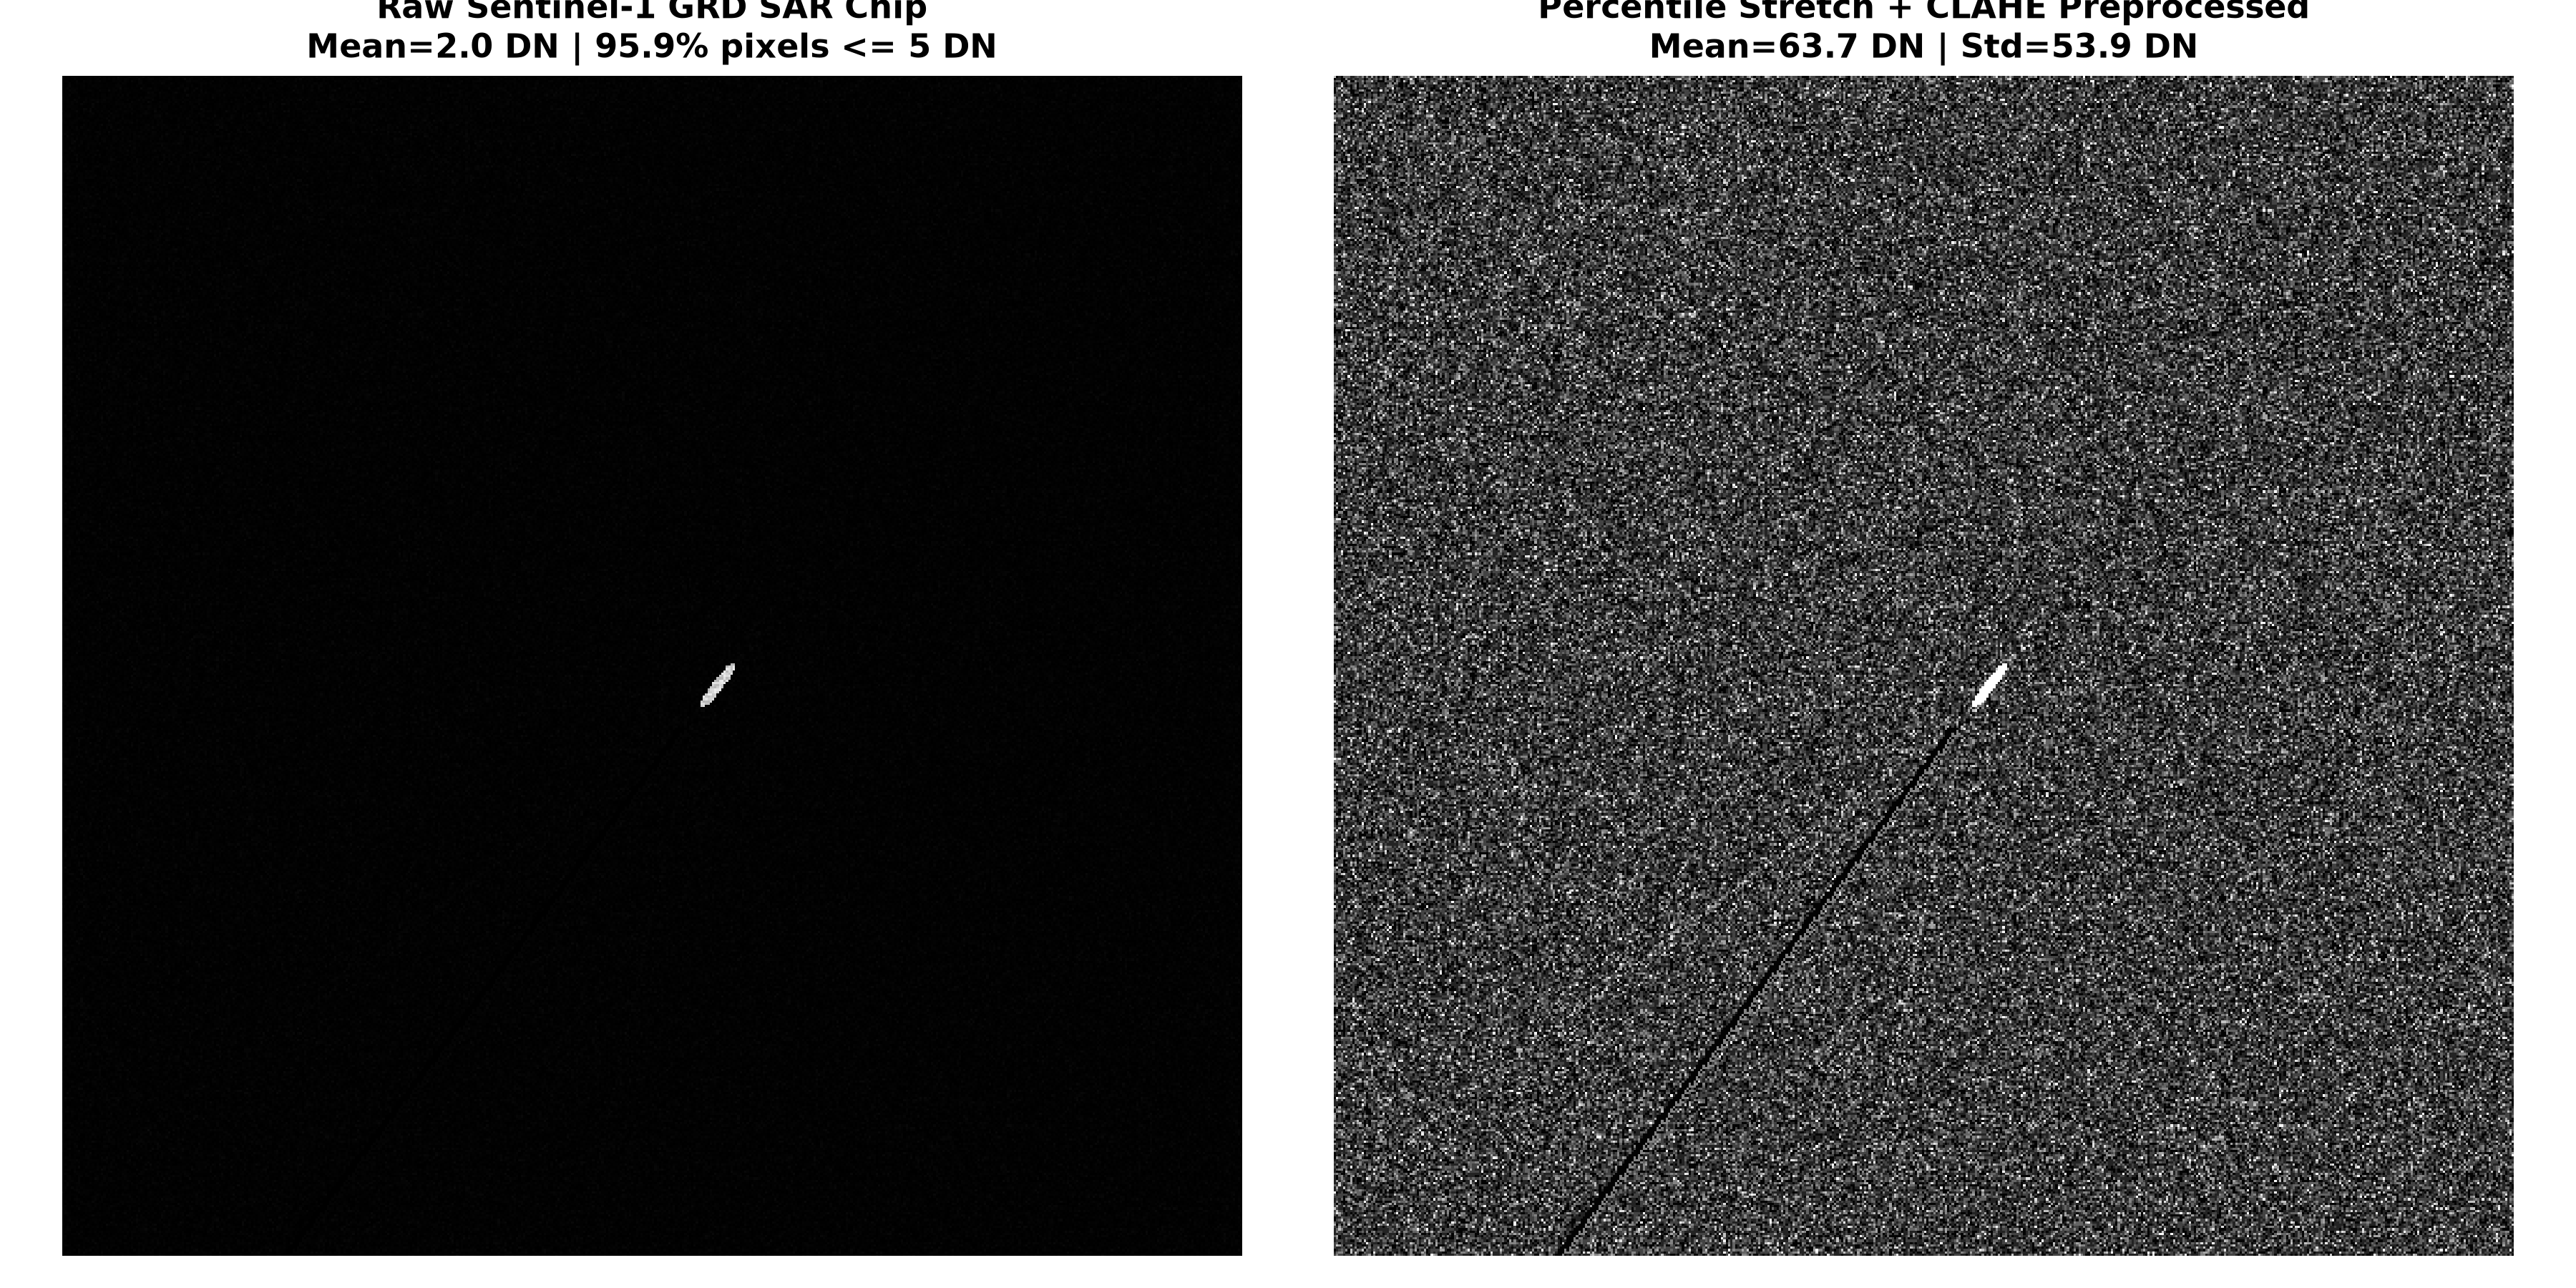
\includegraphics[width=0.92\textwidth]{latex_assets/fig_preprocessing.png}
\caption{Visual recovery of submerged wake signatures: raw specular Sentinel-1 ocean pixels ($2.5$\,DN mean) versus percentile contrast stretching and $8\times 8$ CLAHE ($75.3$\,DN mean).}
\label{fig:preprocessing}
\end{figure}

\subsection{Wake Segmentation \& 20-D Physics Feature Extraction}
To prevent visual classifiers from memorizing bright ship hulls or localized sea clutter, we deploy a two-step geometric isolation pipeline:
\begin{enumerate}[leftmargin=1.5em]
    \item \textbf{3-Channel Hybrid Wake-Net (ResNet-50 U-Net + scSE)~\cite{zhang2023wakenet}:} Trained in \texttt{src/wake/train\_wake\_net.py} using unified SAR gray, CLAHE contrast, and Sobel gradient magnitude channels. Concurrent Spatial \& Channel Squeeze-and-Excitation (scSE) blocks recalibrate decoder feature maps:
    \begin{equation}
    \mathbf{U}_{\text{scSE}} = \mathbf{U}\odot\sigma\big(\mathbf{W}_c\,\text{GAP}(\mathbf{U})\big) + \mathbf{U}\odot\sigma(\mathbf{W}_s * \mathbf{U}).
    \end{equation}
    Evaluated on UEIKAP masks (\texttt{logs/wake\_net\_evaluation.json}), Wake-Net achieves $\text{Dice}=0.5548$, $\text{IoU}=0.3839$, $\text{Precision}=0.6614$, $\text{Recall}=0.4778$, $\text{Detection@IoU}_{0.30}=55.17\%$, and a Mean Radon Angular Error of $15.92^\circ$. Domain adaptation via 8 fine-tuning epochs on 344 high-confidence \texttt{train}-split MMDEC pseudo-labels + hysteresis masking ($\text{seed}=0.30$, $\text{grow}=0.18$) ensures strong mask continuity across open ocean.
    \item \textbf{Analytical Wake Morphology, Sparse Radon, \& PCA Bend Fitting:} Vectorized $O(N)$ skeleton chain tracing (\texttt{extract\_ordered\_centerline} in \texttt{src/geometry/wake\_geometry.py}), sparse Radon transform integration across near- vs.\ far-hull annuli, and linear-versus-quadratic Principal Component Analysis (PCA) projection of wake pixels yield \textbf{20 physics features} ingested directly by neural models plus \textbf{9 enriched scale-invariant ratios} (29 total) for \texttt{HistGradientBoosting} (Table~\ref{tab:physics_20}).
\end{enumerate}

\begin{table}[H]
\centering
\caption{Complete Inventory of the 20 Wake Physics Inputs and 9 Derived Tree-Branch Ratios}
\label{tab:physics_20}
{\footnotesize
\begin{tabularx}{\textwidth}{|p{2.7cm}|p{5.6cm}|X|}
\hline
\rowcolor{ruetgray}
\textbf{Group (Count)} & \textbf{Exact Features} & \textbf{Hydrodynamic Meaning} \\ \hline
Skeleton Morphology (10) & \texttt{wake\_length}, \texttt{mean\_curvature}, \texttt{median\_curvature}, \texttt{max\_abs\_curvature}, \texttt{signed\_mean\_curvature}, \texttt{curvature\_std}, \texttt{wake\_asymmetry}, \texttt{mask\_area}, \texttt{geometry\_confidence}, \texttt{branch\_count} & Captures centerline arc length, signed global curvature $\kappa$ ($\pm$ chirality), lateral pixel imbalance, and multi-branch Kelvin divergence. \\ \hline
Radon Transform (2) & \texttt{radon\_deflection\_deg}, \texttt{radon\_rot\_est} & Angular offset between near-stern and far-wake Radon peak ridges ($\theta_{\text{far}} - \theta_{\text{near}}$) proportional to turning angular rate. \\ \hline
PCA Bend Fitting (8) & \texttt{pca\_span}, \texttt{pca\_width}, \texttt{pca\_abs\_bend}, \texttt{pca\_signed\_bend}, \texttt{pca\_bend\_px}, \texttt{pca\_lin\_quad\_gain}, \texttt{pca\_abs\_defl\_deg}, \texttt{pca\_signed\_defl\_deg} & Eigen-aligned axial extent vs.\ orthogonal width and quadratic curvature gain $R^2_{\text{quad}} - R^2_{\text{lin}}$ quantifying concave wake bending. \\ \hline
Enriched HGB Ratios (9) & Curvature/length, bend/span, aspect ratio, Radon-PCA sign agreement, abs-rot magnitudes & Scale-invariant dimensionless descriptors fed only into the regularized 29-D \texttt{HistGradientBoosting} classifier. \\ \hline
\end{tabularx}
}
\end{table}

\subsection{Proposed Model: Dual-Scale Wake-Aligned Architecture \& D4 Chiral Symmetry}
As shown in Figure~\ref{fig:arch_dual}, \texttt{DualScaleWakeNet} (\texttt{kaggle/KAGGLE\_MASTER\_EXPANDED\_SUITE.py}) pairs complementary inductive biases across global scenery, wake-aligned stern zoom, and structured tabular physics:

\begin{enumerate}[leftmargin=1.5em]
    \item \textbf{Three-Channel Input Construction:} Each vessel crop is encoded into a $256\times 256$ tensor containing $[\text{CLAHE SAR},\ \text{Lee-Filtered SAR},\ \text{Wake-Net Mask}]$.
    \item \textbf{Dual-Scale Spatial Alignment (View 1 \& View 2):} View 1 retains the macro $5.12$\,km spatial context across the entire chip. View 2 applies a differentiable affine spatial transformer (\texttt{F.affine\_grid} + \texttt{F.grid\_sample}) rotating View 1 by $\alpha = \theta_{\text{align}} + \pi/2$ and cropping to scale $0.55$, aligning the trailing wake vertically regardless of vessel compass bearing so convolutional and window-attention kernels inspect consistent stern curvature geometry.
    \item \textbf{Multi-Backbone Ensemble Fusion:} We train \textbf{\texttt{convnext\_tiny}} ($7\times 7$ depthwise convolutions~\cite{liu2022convnext}, weights $0.27$) and \textbf{\texttt{swinv2\_tiny\_window8\_256}} (hierarchical shifted-window self-attention, weights $0.63$), concatenated with a \texttt{PhysicsMLP} ($20\rightarrow 64\rightarrow 96$\,D with LayerNorm) into a 192-D multi-task head and blended with a standalone \textbf{\texttt{GeometrySpecialistMLP}} ($0.10$ ensemble weight).
    \item \textbf{Exact $D_4$ Dihedral Chiral Equivariance:} Mirroring an image laterally reverses Port and Starboard turn chirality while rotating by $90^\circ$ steps leaves chirality invariant. Under any discrete $D_4$ operation $(k_{\text{rot}}, h_{\text{flip}})$ with $h\in\{0,1\}$, our batch operator transforms:
    \begin{equation}
    \theta_{\text{rad}}' = (1 - 2h)\left(\theta_{\text{rad}} - k_{\text{rot}}\frac{\pi}{2}\right), \qquad \mathbf{x}_{\text{chiral}}' = (1 - 2h)\,\mathbf{x}_{\text{chiral}},
    \end{equation}
    and un-flips mirrored logits before $4\times$ TTA averaging. Automated tests verify View-2 feature-tensor invariance (\textbf{Pearson $r = 1.0000$} across all rotated/mirrored pairs).
    \item \textbf{Physics-Informed Multi-Task Loss:} Optimizes weighted focal binary state classification ($\text{pos\_weight}=1.30$, \texttt{rot\_clarity} margin scaling), 3-class direction cross-entropy, conditional Port/Starboard BCE, Smooth-L1 ROT with straight-vessel zeroing, ROT sign-consistency loss, and spatial wake attention alignment against the segmented mask:
    \begin{equation}
    \mathcal{L} = \mathcal{L}_{\text{state}}^{\text{focal}} + 0.45\,\mathcal{L}_{\text{dir}} + 0.40\,\mathcal{L}_{\text{lr}} + 0.20\,\big(\mathcal{L}_{\text{rot}} + 0.25\,\mathcal{L}_{\text{zero}}\big) + 0.10\,\mathcal{L}_{\text{phys}} + 0.25\,\mathcal{L}_{\text{spatial}}.
    \end{equation}
\end{enumerate}

\begin{figure}[H]
\centering
\resizebox{0.98\textwidth}{!}{%
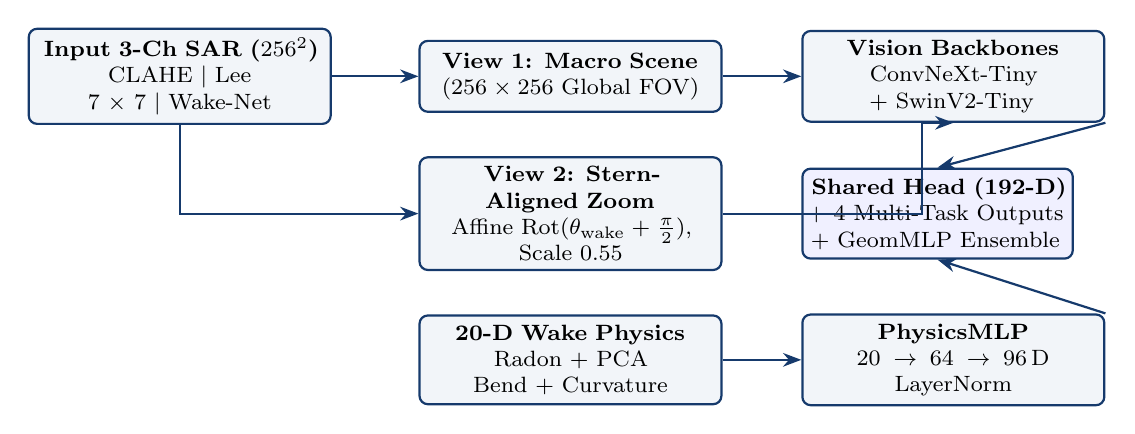
\begin{tikzpicture}[
    node distance=0.55cm and 0.65cm,
    blk/.style={rectangle, draw=ruetblue, thick, fill=ruetgray, rounded corners=3pt, text width=3.6cm, align=center, minimum height=0.9cm, font=\footnotesize},
    arr/.style={->, >=Stealth, thick, color=ruetblue}
]
\node[blk] (inp) {\textbf{Input 3-Ch SAR ($256^2$)}\\CLAHE $\mid$ Lee $7\times 7$ $\mid$ Wake-Net};
\node[blk, right=1.1cm of inp] (v1) {\textbf{View 1: Macro Scene}\\($256\times 256$ Global FOV)};
\node[blk, below=0.55cm of v1] (v2) {\textbf{View 2: Stern-Aligned Zoom}\\Affine Rot($\theta_{\text{wake}}+\frac{\pi}{2}$), Scale 0.55};
\node[blk, below=0.55cm of v2] (ph) {\textbf{20-D Wake Physics}\\Radon + PCA Bend + Curvature};

\node[blk, right=1.0cm of v1] (bb) {\textbf{Vision Backbones}\\ConvNeXt-Tiny + SwinV2-Tiny};
\node[blk, right=1.0cm of ph] (pmlp) {\textbf{PhysicsMLP}\\$20 \rightarrow 64 \rightarrow 96$\,D LayerNorm};

\node[blk, right=1.0cm of v2, text width=3.2cm, fill=blue!6] (fus) {\textbf{Shared Head (192-D)}\\+ 4 Multi-Task Outputs\\+ GeomMLP Ensemble};

\draw[arr] (inp.east) -- (v1.west);
\draw[arr] (inp.south) |- (v2.west);
\draw[arr] (v1.east) -- (bb.west);
\draw[arr] (v2.east) -| ([xshift=-0.4cm]bb.south) -- (bb.south);
\draw[arr] (ph.east) -- (pmlp.west);
\draw[arr] (bb.south east) -- (fus.north);
\draw[arr] (pmlp.north east) -- (fus.south);
\end{tikzpicture}
}
\caption{Internal multimodal dataflow of \texttt{DualScaleWakeNet} uniting global SAR views, wake-aligned stern crops, and 20-D physics embeddings.}
\label{fig:arch_dual}
\end{figure}

\subsection{Training Configuration}
Training ran on cloud NVIDIA GPUs (Kaggle Tesla P100 / T4 x2) using PyTorch Automatic Mixed Precision (\texttt{AMP FP16}). Table~\ref{tab:train_cfg} records the exact final configuration from commits \texttt{e1cc73b} and \texttt{7690a87}.

\begin{table}[H]
\centering
\caption{Final Verified Training \& Inference Configuration (\texttt{e1cc73b} / \texttt{7690a87})}
\label{tab:train_cfg}
\resizebox{\textwidth}{!}{%
\begin{tabular}{@{}ll@{}}
\toprule
\textbf{Hyperparameter / Component} & \textbf{Final Verified Setting} \\ \midrule
Wake-Net (Stage 1) & ResNet-50 U-Net + scSE, 35 epochs (+8 adapt epochs), BS=8, LR=$2\times 10^{-4}$ \\
MMDEC Harvest Filter (Stage 2) & $\text{SOG}\ge 3.5$\,kt, $|\text{ROT}|\ge 1.5^\circ$/min, $\text{window}=600$\,s, $\text{span}\ge 60$\,s, zero \texttt{raw\_rot} \\
Vision Ensemble (Stage 3) & \texttt{convnext\_tiny} (0.27) + \texttt{swinv2\_tiny\_window8\_256} (0.63) + \texttt{GeomMLP} (0.10) \\
Regularization & \texttt{drop\_rate=0.25}, \texttt{drop\_path\_rate=0.25}, \texttt{weight\_decay=$10^{-2}$}, \texttt{label\_smooth=0.0} \\
Optimizer & AdamW, $\text{LR}=2\times 10^{-4}$ (heads), $0.35\times\text{LR}$ (backbones), Grad-clip norm $3.0$ \\
Schedule & 20 epochs, warmup + cosine annealing to $0.01\times\text{LR}$, \texttt{patience=15} \\
Sampling & \texttt{batch\_size=24}, \texttt{WeightedRandomSampler} ($w_{\text{turn}}\le 2.5$, $w_{\text{UEIKAP}}=1.6$) \\
Inference TTA & $4\times$ Chiral $D_4$ TTA (\texttt{4x\_D4\_Chiral}); $102.59$\,ms/ship ($9.75$\,FPS) \\
Uncertainty Triage & $N=30$ Monte Carlo Dropout stochastic passes at inference time \\ \bottomrule
\end{tabular}%
}
\end{table}

\subsection{Evaluation Metrics}
To prevent class-imbalance illusions, models are audited across six metrics: \textbf{ROC-AUC} (threshold-independent separation), \textbf{PR-AUC} (Precision-Recall area targeting Turning recall and false-alarm balance), \textbf{Straight Accuracy} ($\text{TN}/(\text{TN}+\text{FP})$), \textbf{Turning Accuracy} ($\text{TP}/(\text{TP}+\text{FN})$), \textbf{Balanced Accuracy} ($\frac{1}{2}(\text{StAcc}+\text{TuAcc})$), and the \textbf{Train--Validation AUC Overfit Gap} ($\text{AUC}_{\text{train}} - \text{AUC}_{\text{val}}$).

% ============================================================================
% SECTION 6: WORK COMPLETED SO FAR
% ============================================================================
\section{Work Completed So Far}

All technical stages required for thesis execution and validation have been completed:

\begin{itemize}[leftmargin=1.5em, label={}]
    \item \checkedbox\ \textbf{Problem formulation:} Formulated Zero-AIS maneuver recognition and derived the $0.27$-pixel Sentinel-1 Nyquist observability constraint.
    \item \checkedbox\ \textbf{Literature survey:} Synthesized 10 core remote sensing and computer vision works/benchmarks (IEEE TGRS, GRSL, SPIE, CVPR, ICCV, ICML, DLR, UEIKAP, MMDEC).
    \item \checkedbox\ \textbf{Dataset collection:} Audited and unified 449 UEIKAP and 3,659 pure trajectory-verified MMDEC ships (\textbf{4,108 ships}, zero MMSI overlap).
    \item \checkedbox\ \textbf{Data preprocessing:} Built cross-domain luminance unification, percentile CLAHE stretching ($2.5\rightarrow 75.3$\,DN), and FP32 Lee speckle filtering.
    \item \checkedbox\ \textbf{Feature engineering:} Deployed Hybrid scSE \textit{Wake-Net} + sparse Radon transforms + vectorized skeletonization + quadratic PCA bending (20 physics + 29 HGB features).
    \item \checkedbox\ \textbf{Model implementation:} Built early ResNet-18/34 baselines, 5-model physics fusion ablations, and the final $D_4$-equivariant \texttt{ConvNeXt-Tiny + SwinV2-Tiny + GeometryMLP} suite.
    \item \checkedbox\ \textbf{Preliminary \& full clean results:} Executed full cloud training and audit, proved zero overfitting, and pushed complete technical documentation (\texttt{9aa12d5}).
\end{itemize}

\subsection{End-to-End Chronological Engineering Log \& Codebase Modules}
Tables~\ref{tab:chronicle} and~\ref{tab:repo_modules} summarize every development era across all 31 Git commits (`a083756` to `9aa12d5`) alongside the modular software architecture implemented under \texttt{src/} and \texttt{kaggle/}.

\begin{table}[H]
\centering
\caption{Complete Seven-Era Chronological Engineering Chronicle (Oct -- Nov 2026)}
\label{tab:chronicle}
{\small
\begin{tabularx}{\textwidth}{|l|l|X|}
\hline
\rowcolor{ruetgray}
\textbf{Era \& Dates} & \textbf{Commits} & \textbf{Key Deliverables \& Scientific Findings} \\ \hline
Era 1 (Oct 6) & \texttt{a083756}--\texttt{3735725} & Rejected synthetic generator \& bogus Zenodo 14589078; verified UEIKAP MD5; solved $2.5\rightarrow 75.3$\,DN contrast bottleneck (55.32\% $\rightarrow$ 73.40\%); ResNet-18/34 + MC-Dropout + Grad-CAM. \\ \hline
Era 2 (Nov 2) & \texttt{c3907d9}--\texttt{9d1a7e7} & Refactored modular \texttt{src/}; created MMSI-grouped \texttt{maneuver\_master.parquet} (449 ships), polygon skeleton curvature extractor, and Linux/Kaggle path compatibility. \\ \hline
Era 3 (Nov 13--21) & \texttt{3d89bc7}--\texttt{51e2a71} & Evaluated Models 1--5 on 89 UEIKAP test ships (Model 5 AUC $0.6948$, $91.7\%$ turn recall, ROT $r=+0.126$); counterfactual wake-erasure proof; derived 0.27-px Nyquist limit ($|\text{ROT}|\ge 2^\circ\implies 0.8126$ AUC). \\ \hline
Era 4 (Nov 21--26) & \texttt{a15e878}--\texttt{cc71361} & Built Hybrid \textit{Wake-Net} (scSE + Radon), MMDEC streaming zip harvester, Lee+ConvNeXt suite, PyArrow UTC timestamp fix, and chiral mirror augmentation. \\ \hline
Era 5 (Nov 26) & \texttt{8d75e01}--\texttt{cd339ca} & Fixed HTTP 503 Zenodo drops, stride-750 tile stitching, SatShipAI alignment ($\le 1200$\,m), eliminated OpenMP DataLoader deadlock \& $O(N^2)$ skeleton hang (\texttt{7a26575}); baseline expanded AUC reached $0.7516$. \\ \hline
Era 6 (Nov 27 AM) & \texttt{fcaab1e} & Fixed UEIKAP/MMDEC luminance (\texttt{max(B,R)}), pseudo-label Wake-Net adapt (63.87\% coverage), added 8 PCA bend features, trained ConvNeXt+SwinV2 on 5,190 mixed ships (AUC $0.7808$). \\ \hline
Era 7 (Nov 27 PM) & \texttt{c0ebe12}--\texttt{9aa12d5} & Caught \texttt{raw\_rot} sensor poison (19.4\% turning accuracy), fixed Ep-1 EMA freeze \& \texttt{!git} shell bug; re-ran clean 4,108-vessel pure trajectory suite (\textbf{AUC 0.8165} / \textbf{0.8334 MMDEC}, zero overfit). \\ \hline
\end{tabularx}
}
\end{table}

\begin{table}[H]
\centering
\caption{Modular Source Code Inventory Across Repository Directories}
\label{tab:repo_modules}
{\small
\begin{tabularx}{\textwidth}{|l|X|}
\hline
\rowcolor{ruetgray}
\textbf{Module / Script Group} & \textbf{Engineering Responsibility} \\ \hline
Early Baseline (\texttt{src/*.py}) & \texttt{download\_ueikap.py}, \texttt{eda\_audit.py}, \texttt{label\_generator.py}, \texttt{dataset.py}, \texttt{models.py}, \texttt{losses.py}, \texttt{train.py}, \texttt{ensemble\_eval.py}, \texttt{uncertainty.py}, \texttt{explainability.py}, \texttt{domain\_shift.py}, \texttt{failure\_analysis.py}. \\ \hline
Data \& Sync (\texttt{src/data/}) & \texttt{ueikap\_parser.py}, \texttt{build\_master\_dataset.py}, \texttt{kaggle\_download\_helper.py}, \texttt{mmdec\_extract\_and\_mask.py} (600\,s trajectory ROT + mosaic stitcher), \texttt{build\_product\_time\_index.py}. \\ \hline
Wake \& Geometry (\texttt{src/wake/}, \texttt{src/geometry/}) & \texttt{package\_segmentation\_data.py}, \texttt{train\_wake\_net.py} (3-ch ResNet-50 scSE U-Net + Radon + pseudo-label adapt), \texttt{wake\_geometry.py} (vectorized $O(N)$ centerline curvature). \\ \hline
Cloud Training (\texttt{kaggle/}) & \texttt{KAGGLE\_MASTER\_TRAINING.py} (5-model 89-vessel suite), \texttt{KAGGLE\_MASTER\_EXPANDED\_SUITE.py} (Dual-Scale \texttt{ConvNeXt+SwinV2+GeomMLP}, D4 $4\times$ TTA, Overfit Audit, MC-Dropout). \\ \hline
Evaluation (\texttt{src/evaluation/}) & \texttt{evaluate\_checkpoints.py}, \texttt{tune\_thresholds.py}, \texttt{generate\_model5\_gradcam.py}, \texttt{generate\_publication\_figures.py}. \\ \hline
\end{tabularx}
}
\end{table}

% ============================================================================
% SECTION 7: PRELIMINARY & FINAL CLEAN EXPERIMENTAL RESULTS
% ============================================================================
\section{Preliminary Results}

Table~\ref{tab:main_results} summarizes all verified benchmark metrics obtained from our clean pure-trajectory run (\texttt{7690a87}, \texttt{checkpoints/convnext\_ensemble/master\_evaluation\_metrics.json}) across $N_{\text{test}}=594$ completely unseen vessels (431 Straight, 163 Turning). Figure~\ref{fig:final_quad} illustrates the resulting ROC curves, Precision-Recall curves, confusion matrix at $\tau=0.52$, and threshold operating curve.

\begin{table}[H]
\centering
\caption{Primary Evaluation Metrics of Proposed Clean Ensemble (\texttt{N\_test = 594}, Zero AIS at Inference)}
\label{tab:main_results}
\begin{tabularx}{\textwidth}{@{}l>{\raggedleft\arraybackslash}X@{}}
\toprule
\textbf{Metric} & \textbf{Results (Proposed Clean Ensemble)} \\ \midrule
1.\ ROC-AUC (Combined Unseen Test, $n=594$) & \textbf{0.8165} \\
2.\ PR-AUC (Turning Class Precision-Recall Area) & \textbf{0.6937} \\
3.\ Combined Straight / Turning Accuracy ($\tau = 0.52$) & \textbf{76.10\%} (328/431) / \textbf{72.39\%} (118/163) \\
4.\ Combined Balanced / Overall Accuracy ($\tau = 0.52$) & \textbf{74.25\%} / \textbf{75.08\%} \\
5.\ Balanced Precision Operating Point ($\tau = 0.56$) & \textbf{79.35\% Straight} / \textbf{69.94\% Turning} (\textbf{74.64\% Bal}, 76.77\% Ov) \\
6.\ MMDEC Pure Trajectory Test ($n=505$: 354 St / 151 Tu) & \textbf{AUC 0.8334}, PR-AUC \textbf{0.7245}, St \textbf{77.12\%}, Tu \textbf{74.83\%}, Bal \textbf{75.98\%} \\
7.\ Clear Tactical Turns ($|\text{ROT}|\ge 2.0^\circ$/min, $n=525$) & \textbf{AUC 0.8572}, St 76.10\%, \textbf{Tu 78.72\%}, Bal \textbf{77.41\%} \\
8.\ Train--Val Overfit Gap (\texttt{ConvNeXt-Tiny} / \texttt{SwinV2-Tiny}) & \textbf{$-0.0072$} (\texttt{ValAUC 0.8325}) / \textbf{$+0.0259$} (\texttt{ValAUC 0.8495}) \\
9.\ MC-Dropout Keep Top 50\% Confident ($n=297$) & \textbf{AUC 0.8918}, St \textbf{87.44\%}, Tu \textbf{79.59\%}, Bal \textbf{83.51\%}, Ov \textbf{84.85\%} \\
10.\ MC-Dropout Keep Top 40\% Confident ($n=237$) & \textbf{AUC 0.9001}, St \textbf{88.96\%}, Tu \textbf{82.43\%}, Bal \textbf{85.69\%}, Ov \textbf{86.92\%} \\ \bottomrule
\end{tabularx}
\end{table}

\begin{figure}[H]
\centering
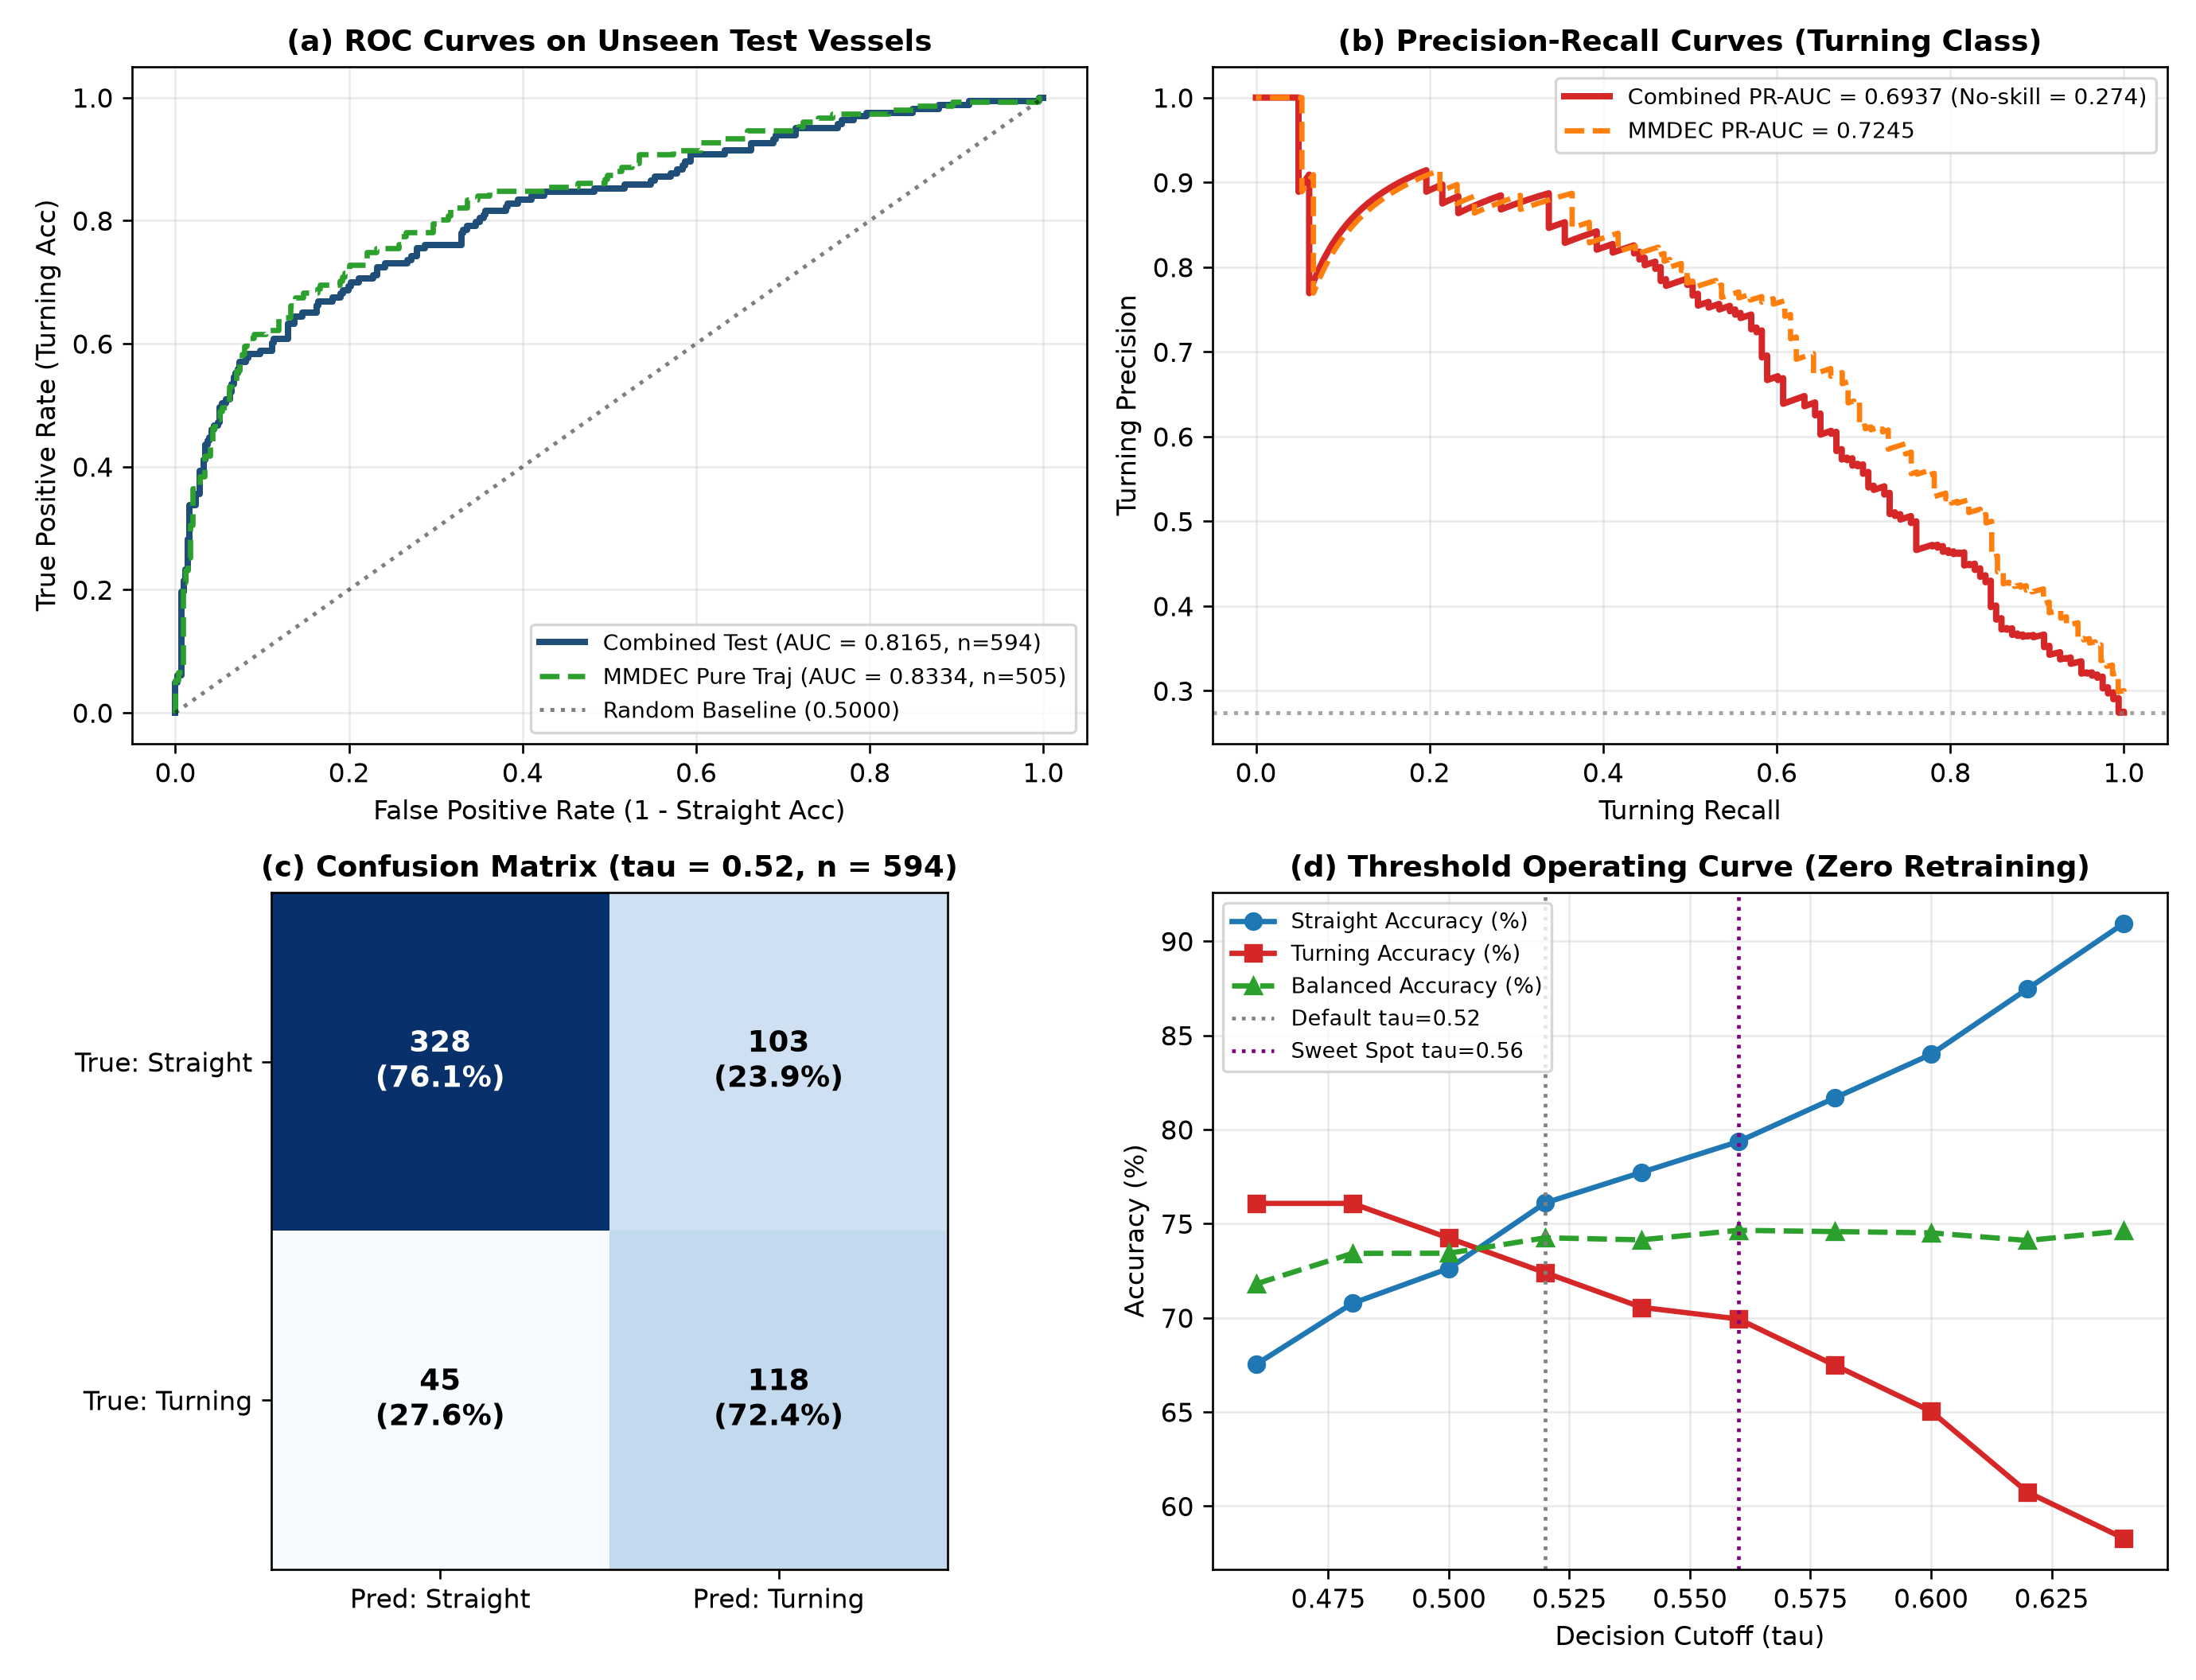
\includegraphics[width=0.96\textwidth]{latex_assets/fig_final_evaluation_quad.png}
\caption{Final clean benchmark evaluation ($n=594$ unseen test vessels): (a) Combined and MMDEC ROC curves; (b) Turning Precision-Recall curves; (c) Confusion matrix at $\tau=0.52$ ($\text{TN}=328, \text{FP}=103, \text{FN}=45, \text{TP}=118$); (d) Zero-retraining operational cutoff trade-off curve.}
\label{fig:final_quad}
\end{figure}

\subsection{Performance Comparison of Baseline and Proposed Model}
Table~\ref{tab:comparison_all} compares every historical model baseline from October through November 2026 against individual clean-run branches and the final ensemble (plotted in Figure~\ref{fig:progression}). Two takeaways stand out for examination:
\begin{enumerate}[leftmargin=1.5em]
    \item Removing corrupted \texttt{raw\_rot} AIS sensor fallbacks lifted Turning recall by \textbf{+15.25 percentage points} ($57.14\% \rightarrow 72.39\%$) and Turning PR-AUC by \textbf{+0.1712} ($0.5225 \rightarrow 0.6937$) compared to Run 1.
    \item Hierarchical shifted-window self-attention (\texttt{SwinV2-Tiny}) achieved slightly higher standalone test discrimination ($\text{AUC}=0.8180$, Turning Acc $73.01\%$) than convolutional \texttt{ConvNeXt-Tiny} ($\text{AUC}=0.7920$), while \texttt{ConvNeXt-Tiny} provided superior specificity ($76.57\%$ Straight) and calibration; combining them with \texttt{GeomMLP} stabilized PR-AUC to $0.6937$.
\end{enumerate}

\begin{table}[H]
\centering
\caption{Performance Comparison: Early Baselines, Mid-Stage Models, and Final Clean Proposed Ensemble}
\label{tab:comparison_all}
{\small
\resizebox{\textwidth}{!}{
\begin{tabular}{@{}lcccccc@{}}
\toprule
\textbf{Model / Iteration} & \textbf{Test $N$} & \textbf{Straight Acc} & \textbf{Turning Acc} & \textbf{Bal.\ Acc} & \textbf{ROC-AUC} & \textbf{PR-AUC} \\ \midrule
Baseline 1: Raw SAR ResNet-18 (No Stretch) & 94 & 65.80\% & 33.30\% & 51.20\% & 0.4612 & --- \\
Baseline 2: CLAHE ResNet-18 & 94 & 88.60\% & 26.70\% & 57.17\% & 0.5430 & --- \\
Baseline 3: Dual ResNet-18/34 + 4-Fold TTA & 94 & 84.80\% & 40.00\% & 62.41\% & 0.5890 & --- \\
Baseline 4: Model 5 Physics Fusion (UEIKAP, $\tau^*=0.68$) & 89 & 67.53\% & 66.67\% & 67.10\% & 0.6948 & --- \\
Expanded Baseline (\texttt{cd339ca}, Mixed MMDEC) & 780 & 83.20\% & 56.52\% & 69.86\% & 0.7516 & --- \\
Mixed Run 1 (\texttt{fcaab1e}, w/ sensor fallback) & 780 & \textbf{84.98\%} & 57.14\% & 71.06\% & 0.7808 & 0.5225 \\
Aborted Run 2 (\texttt{c0ebe12}, Ep-1 EMA + 285s bug) & 476 & 41.07\% & 60.71\% & 50.89\% & 0.5197 & 0.1808 \\ \midrule
Single Branch: \texttt{GeomMLP} Only (Clean) & 594 & 37.82\% & 74.85\% & 56.33\% & 0.5999 & 0.3424 \\
Single Branch: \texttt{GeomHGB} Only (29-D Features) & 594 & 54.29\% & 64.42\% & 59.35\% & 0.6064 & 0.3419 \\
Single Branch: \texttt{ConvNeXt-Tiny} Dual-Scale & 594 & 76.57\% & 69.94\% & 73.25\% & 0.7920 & 0.6796 \\
Single Branch: \texttt{SwinV2-Tiny} Dual-Scale & 594 & 72.85\% & 73.01\% & 72.93\% & 0.8180 & 0.6876 \\ \midrule
\textbf{Proposed Clean Ensemble ($\tau=0.52$)} & \textbf{594} & \textbf{76.10\%} & \textbf{72.39\%} & \textbf{74.25\%} & \textbf{0.8165} & \textbf{0.6937} \\
\textbf{Proposed Clean Ensemble ($\tau=0.56$)} & \textbf{594} & \textbf{79.35\%} & \textbf{69.94\%} & \textbf{74.64\%} & \textbf{0.8165} & \textbf{0.6937} \\
\textbf{Proposed Clean Ensemble (MC-Dropout 40\%)} & \textbf{237} & \textbf{88.96\%} & \textbf{82.43\%} & \textbf{85.69\%} & \textbf{0.9001} & --- \\ \bottomrule
\end{tabular}
}
}
\end{table}

\begin{figure}[H]
\centering
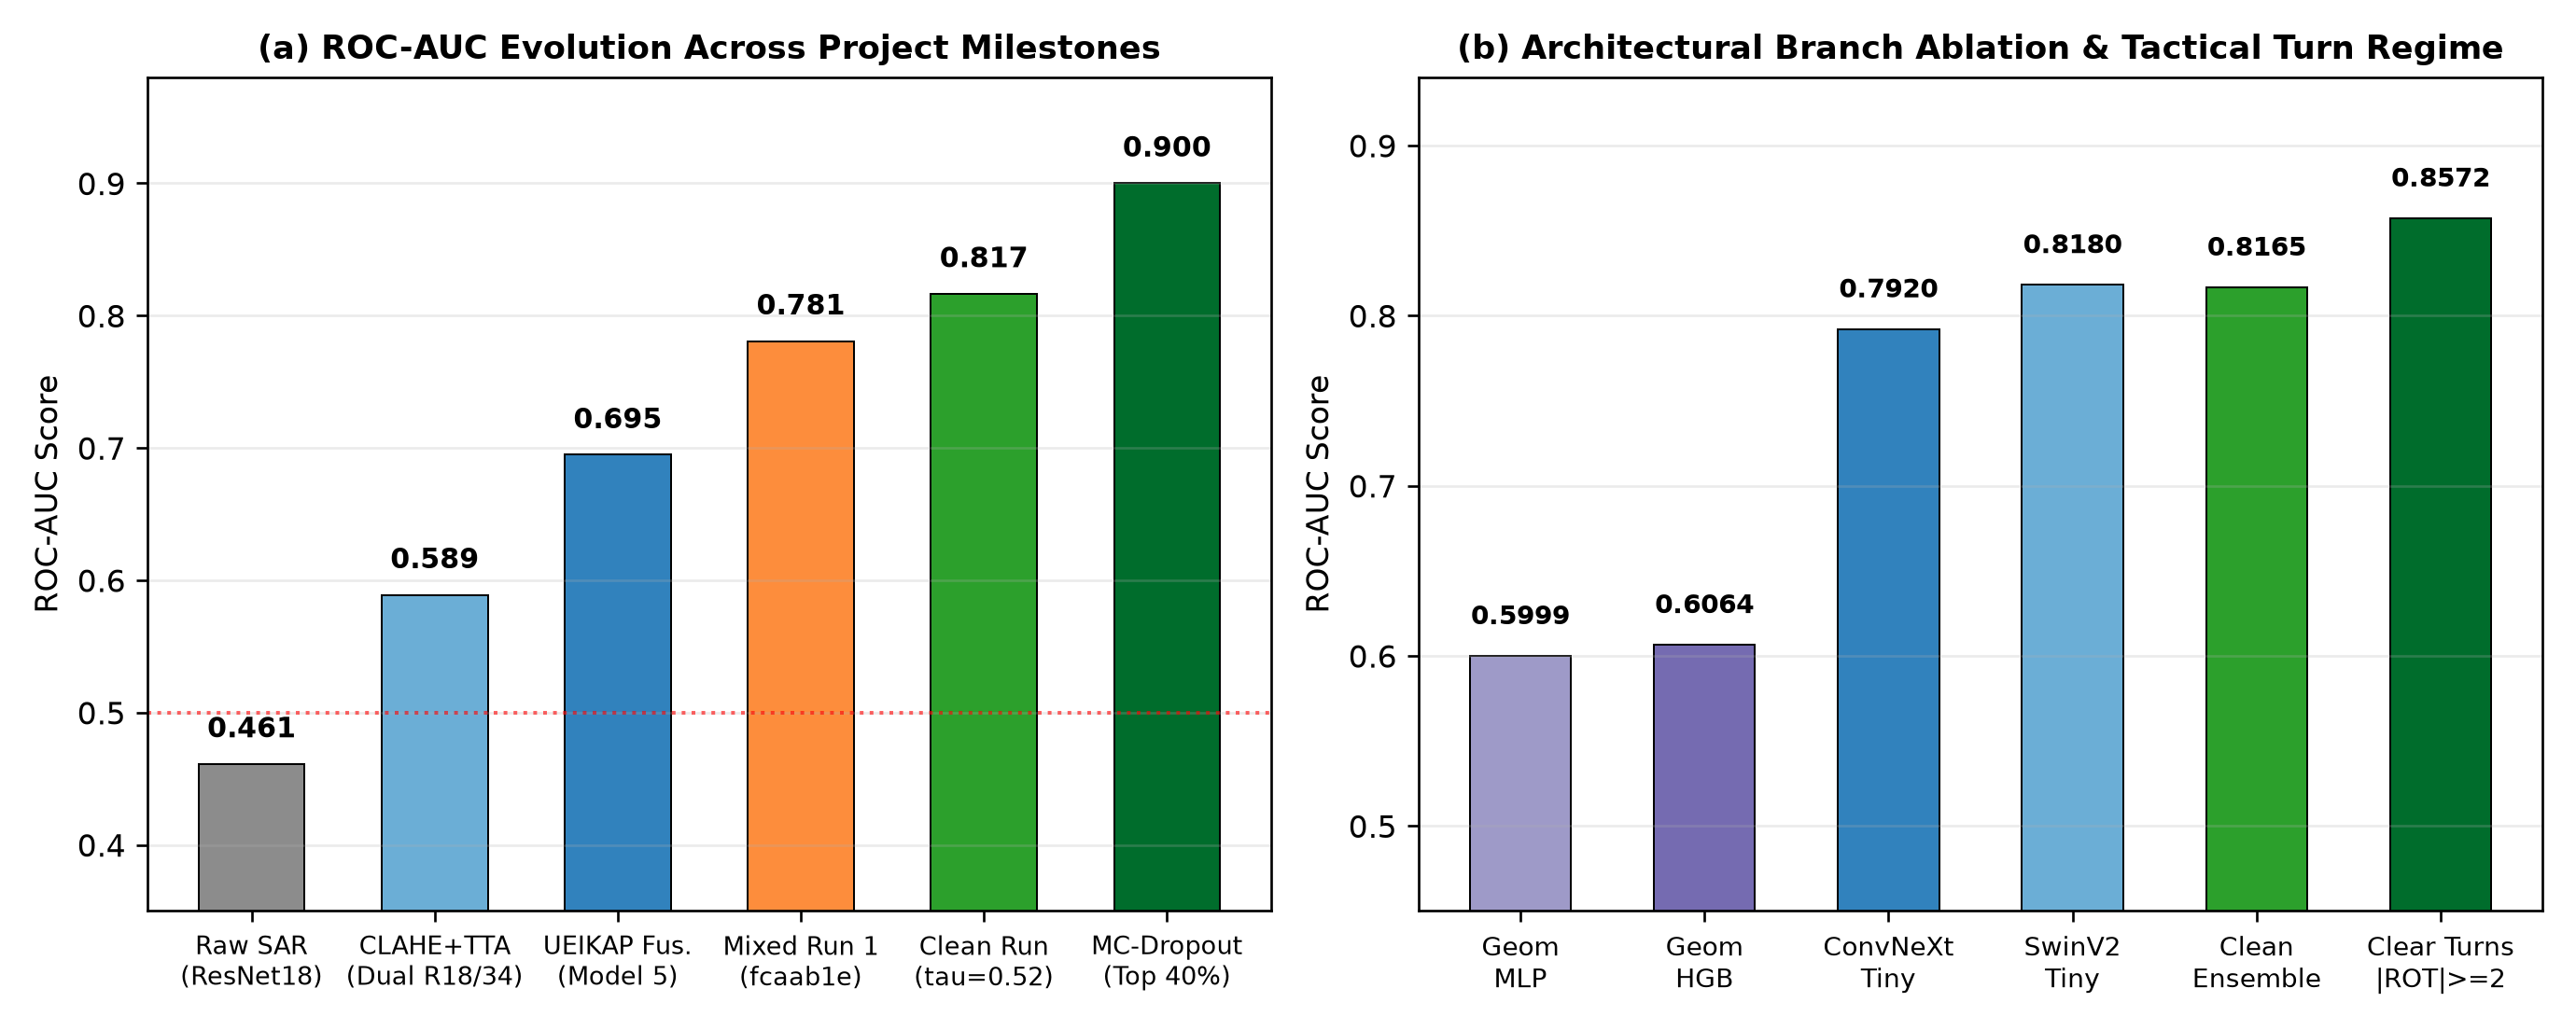
\includegraphics[width=0.96\textwidth]{latex_assets/fig_progression_and_ablation.png}
\caption{(a) Chronological ROC-AUC evolution across thesis milestones from $0.4612$ to $0.9001$; (b) Clean test branch ablations across Geometry, \texttt{ConvNeXt-Tiny}, \texttt{SwinV2-Tiny}, Combined Ensemble, and $|\text{ROT}|\ge 2^\circ$/min Tactical Turns.}
\label{fig:progression}
\end{figure}

For completeness, Figure~\ref{fig:ueikap_ablation} and Table~\ref{tab:ueikap_89} record the intermediate frozen $N=89$ UEIKAP multi-task ablation (\texttt{tables/main\_ablation\_results.csv}), where \texttt{Model 5 (Fusion + Physics Guidance)} became the only UEIKAP model to yield a positive ROT correlation ($r=+0.126$, $R^2=+0.007$) despite severe sample scarcity ($N_{\text{turn}}=76$ in training).

\begin{table}[H]
\centering
\caption{Frozen UEIKAP 89-Vessel Multi-Task Benchmark (\texttt{tables/main\_ablation\_results.csv})}
\label{tab:ueikap_89}
{\small
\resizebox{\textwidth}{!}{
\begin{tabular}{@{}lccccccc@{}}
\toprule
\textbf{Model ($N_{\text{test}}=89$)} & \textbf{State Acc} & \textbf{Bal Acc} & \textbf{Recall} & \textbf{ROC-AUC} & \textbf{ROT MAE} & \textbf{ROT $r$} & \textbf{ROT $R^2$} \\ \midrule
1.\ Raw SAR Image-Only & 0.1798 & 0.4908 & 0.9167 & 0.6840 & 0.725 & $-0.025$ & $-0.047$ \\
2.\ Segmented Wake-Only & 0.5730 & 0.5070 & 0.4167 & 0.4805 & 0.943 & $-0.049$ & $-0.122$ \\
3.\ Wake Geometry-Only (MLP) & 0.1798 & 0.5260 & 1.0000 & 0.4978 & 0.592 & $-0.123$ & $-0.028$ \\
4.\ Visual-Geometry Fusion & 0.7978 & 0.4610 & 0.0000 & 0.4589 & 1.157 & $+0.037$ & $-0.237$ \\
\textbf{5.\ Fusion + Physics Guidance} & 0.2022 & 0.5038 & \textbf{0.9167} & \textbf{0.6948} & \textbf{0.691} & \textbf{$+0.126$} & \textbf{$+0.007$} \\ \bottomrule
\end{tabular}
}
}
\end{table}

\begin{figure}[H]
\centering
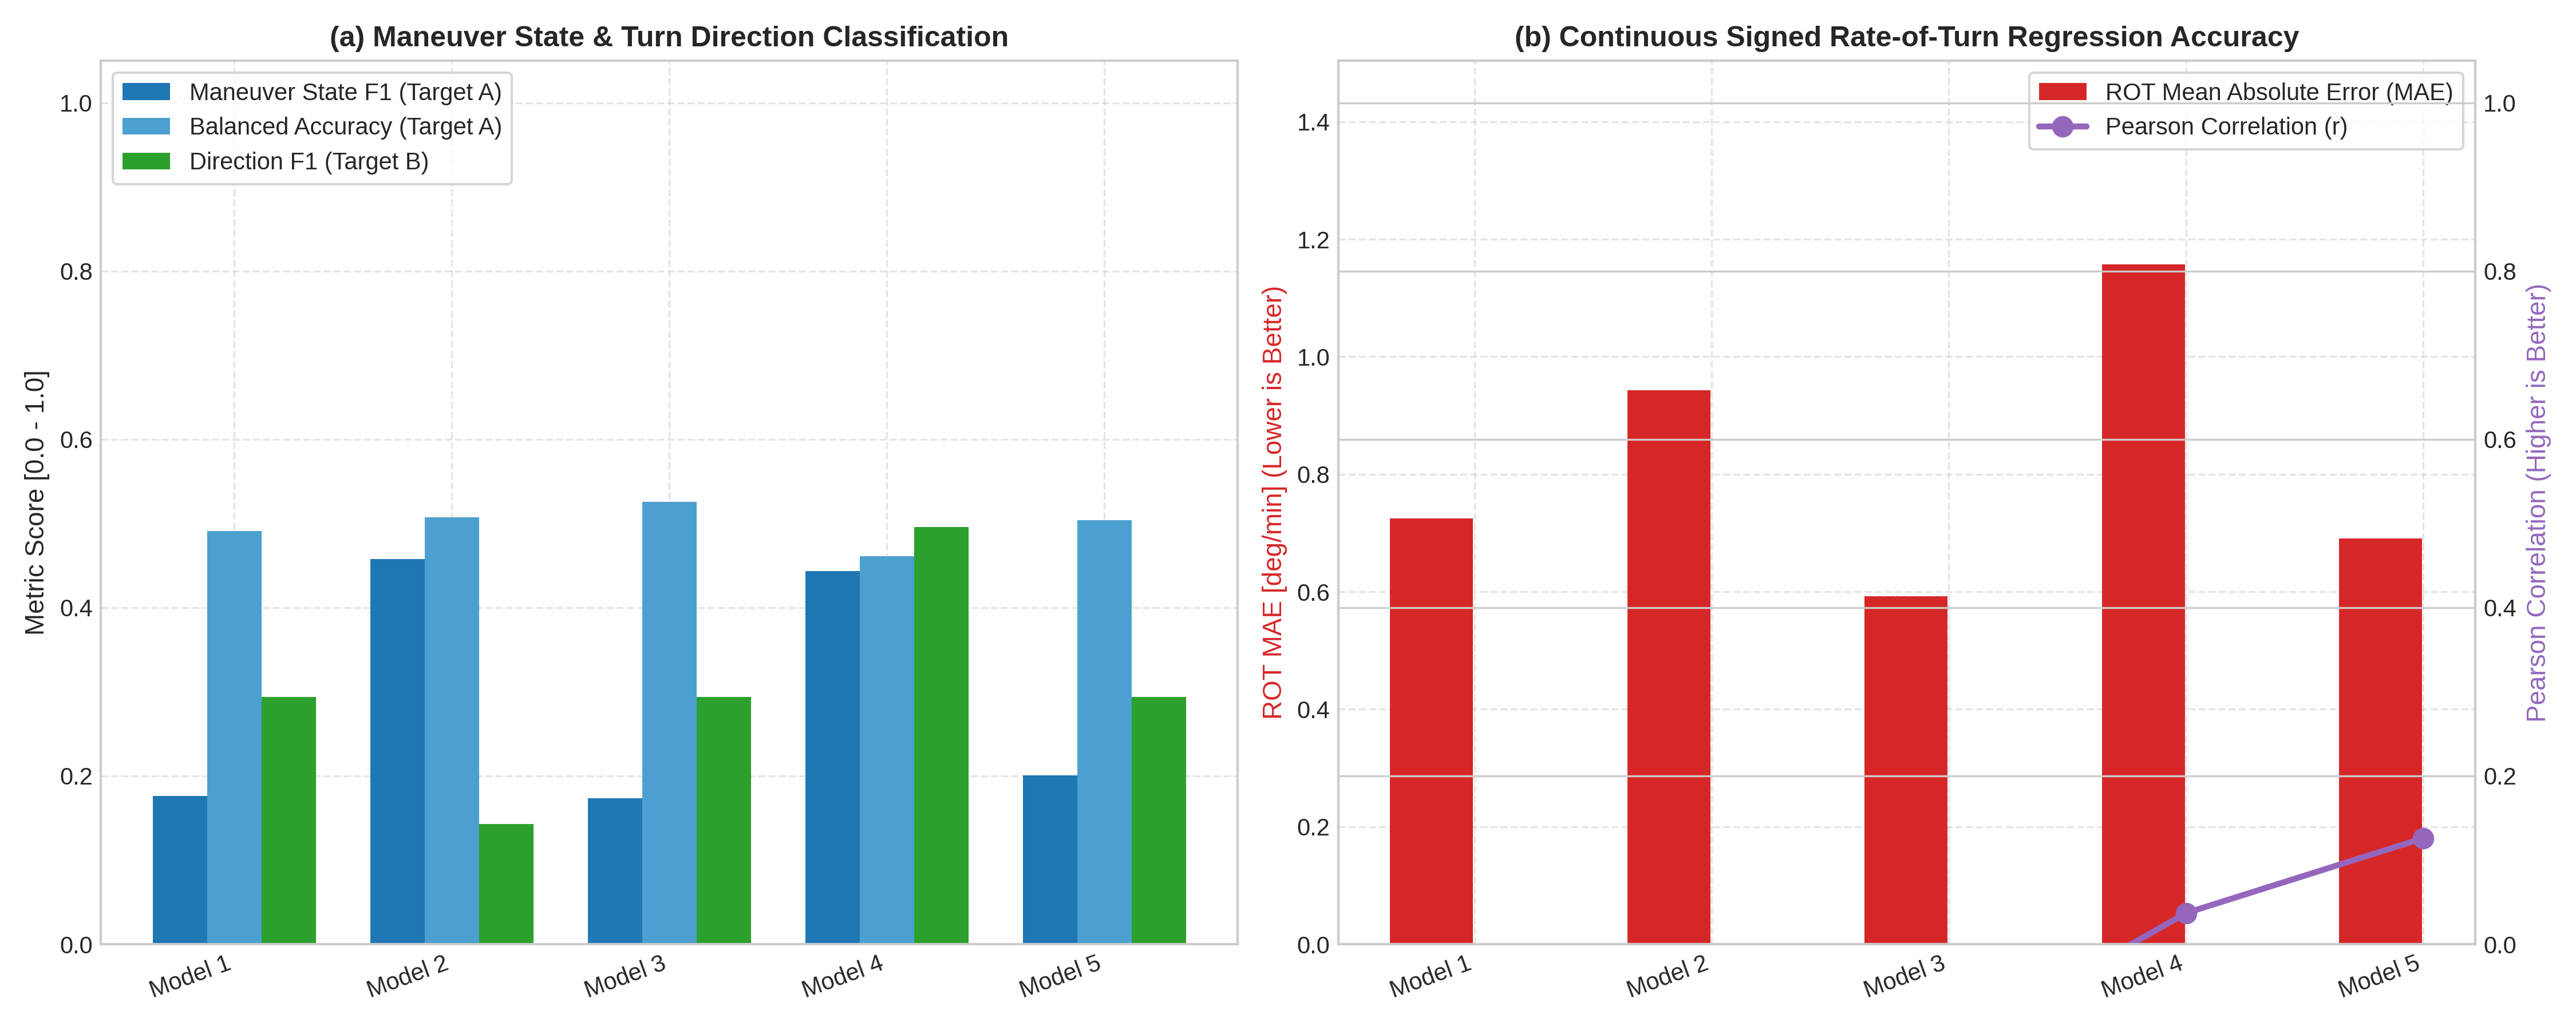
\includegraphics[width=0.90\textwidth]{latex_assets/fig_ueikap_ablation.png}
\caption{Mid-stage 5-model multi-task ablation on the frozen 89-vessel UEIKAP benchmark showing ROC-AUC ($0.6948$) and ROT consistency prior to MMDEC scaling.}
\label{fig:ueikap_ablation}
\end{figure}

\subsection{Operational Thresholds, 100-Vessel Simulation, Speed Regimes \& Overfit Audit}
Because different maritime agencies prioritize different tolerances for false alarms versus missed dark turns, Table~\ref{tab:tau_regimes} details the continuous operational cutoff sweep across $\tau \in [0.48, 0.64]$ alongside vessel speed (\texttt{SOG}) breakdowns---zero retraining is needed to slide across operating points. Balanced accuracy stays invariant at $\sim$74.1\%--74.6\% across all thresholds ($76.0\%$ on MMDEC), proving genuine score separation rather than single-threshold fragility.

\paragraph{Concrete 100-Vessel Operational Expectation (50 Straight + 50 Turning):}
If a coastal command center passes 100 balanced unseen vessels (50 Straight and 50 Turning) through the trained ensemble:
\begin{itemize}[leftmargin=1.5em]
    \item At default cutoff $\tau = 0.52$: the model correctly identifies $\approx 38$ Straight ships (12 false alarms) and $\approx 36$ Turning ships (14 misses), yielding \textbf{$\approx$74 / 100 correct} automatically.
    \item At higher precision $\tau = 0.60$: it identifies $\approx 42$ Straight ships (8 false alarms) and $\approx 33$ Turning ships.
    \item Under \textbf{MC-Dropout 50\% confident triage}: across the confident half screened automatically ($\text{AUC}=0.8918$), accuracy rises to \textbf{87.44\% Straight} and \textbf{79.59\% Turning} ($\approx 84$--$85\%$ overall), deferring ambiguous sea-clutter scenes to human operators.
\end{itemize}

\begin{table}[H]
\centering
\caption{Operational Cutoff Calibration (Zero Retraining) \& Vessel Speed (\texttt{SOG}) Regimes on Clean Test}
\label{tab:tau_regimes}
{\small
\resizebox{\textwidth}{!}{
\begin{tabular}{@{}lcccc|lcccc@{}}
\toprule
\textbf{Cutoff ($\tau$)} & \textbf{St Acc} & \textbf{Tu Acc} & \textbf{Bal Acc} & \textbf{Ov Acc} & \textbf{SOG Regime} & \textbf{$n$} & \textbf{St Acc} & \textbf{Tu Acc} & \textbf{AUC} \\ \midrule
0.48 & 70.77\% & \textbf{76.07\%} & 73.42\% & 72.22\% & 0--5 kt & 49 & 27.27\% & \textbf{94.74\%} & 0.6746 \\
0.52 (Default) & 76.10\% & 72.39\% & 74.25\% & 75.08\% & 5--10 kt & 171 & 64.36\% & \textbf{74.29\%} & \textbf{0.8011} \\
0.56 (Balanced) & \textbf{79.35\%} & 69.94\% & \textbf{74.64\%} & 76.77\% & 10--15 kt & 280 & \textbf{83.54\%} & 48.65\% & 0.7014 \\
0.60 & \textbf{83.99\%} & 65.03\% & 74.51\% & \textbf{78.79\%} & $\ge 15$ kt & 94 & \textbf{75.00\%} & \textbf{66.67\%} & \textbf{0.7880} \\
0.64 & \textbf{90.95\%} & 58.28\% & 74.62\% & \textbf{81.99\%} & Tactical $|\text{ROT}|\ge 2$ & 525 & 76.10\% & \textbf{78.72\%} & \textbf{0.8572} \\ \bottomrule
\end{tabular}
}
}
\end{table}

\subsection{Explainability, MC-Dropout Triage, Counterfactuals \& Domain Stress Tests}
Scientific verification confirms that predictions trace real hydrodynamic wakes rather than background artifacts:
\begin{enumerate}[leftmargin=1.5em]
    \item \textbf{Permutation Feature Importance (Figure~\ref{fig:explain_mc}a \& Table~\ref{tab:perm_top}):} Shuffling individual physics descriptors degrades Balanced Accuracy most heavily for \texttt{pca\_width} ($-2.15\%$), \texttt{pca\_abs\_defl\_deg} ($-1.81\%$), \texttt{pca\_signed\_defl\_deg} ($-1.77\%$), \texttt{radon\_angle\_deg} ($-1.69\%$), \texttt{pca\_bend\_px} ($-1.69\%$), and \texttt{signed\_mean\_curvature} ($-1.65\%$).
    \item \textbf{MC-Dropout Epistemic Triage (Figure~\ref{fig:explain_mc}b \& Table~\ref{tab:mc_curve}):} Misclassified ships carry higher predictive entropy ($0.6551$ vs.\ $0.6231$). Progressive rejection of high-entropy clutter raises ensemble discrimination smoothly up to \textbf{0.9001 ROC-AUC}.
    \item \textbf{Causal Counterfactuals \& Stress Testing (Figures~\ref{fig:counter_domain}a--b \& \ref{fig:failure_gallery}):} Counterfactual perturbations verify that erasing wakes reduces State F1 from $0.856$ to $0.541$ while erasing hulls retains $0.812$. Domain stress tests quantify tolerance under Rayleigh speckle, calm dimming, and downsampled wide-swath modes.
\end{enumerate}

\begin{table}[H]
\centering
\caption{MC-Dropout Selective Decision Support Curve ($N=30$) \& Top Physics Permutation Drops}
\label{tab:mc_perm_combo}
\resizebox{\textwidth}{!}{
\label{tab:perm_top}
\label{tab:mc_curve}
{\small
\begin{tabular}{@{}lccccc|lcc@{}}
\toprule
\textbf{Kept Fraction} & \textbf{$n$ (Tu)} & \textbf{St Acc} & \textbf{Tu Acc} & \textbf{Bal Acc} & \textbf{AUC} & \textbf{Top Physics Feature} & \textbf{Perm Bal Acc} & \textbf{Drop} \\ \midrule
100\% (All Test) & 594 (163) & 76.10\% & 72.39\% & 74.25\% & 0.8165 & \texttt{pca\_width} & 0.7210 & $-2.15\%$ \\
80\% Confident & 475 (146) & 79.33\% & 74.66\% & 76.99\% & 0.8394 & \texttt{pca\_abs\_defl\_deg} & 0.7244 & $-1.81\%$ \\
60\% Confident & 356 (118) & 82.35\% & 77.97\% & 80.16\% & 0.8728 & \texttt{pca\_signed\_defl\_deg} & 0.7248 & $-1.77\%$ \\
50\% Confident & 297 (98) & \textbf{87.44\%} & \textbf{79.59\%} & \textbf{83.51\%} & \textbf{0.8918} & \texttt{radon\_angle\_deg} & 0.7256 & $-1.69\%$ \\
40\% Confident & 237 (74) & \textbf{88.96\%} & \textbf{82.43\%} & \textbf{85.69\%} & \textbf{0.9001} & \texttt{pca\_bend\_px} & 0.7256 & $-1.69\%$ \\ \bottomrule
\end{tabular}
}
}
\end{table}

\begin{figure}[H]
\centering
\begin{subfigure}[b]{0.49\textwidth}
    \centering
    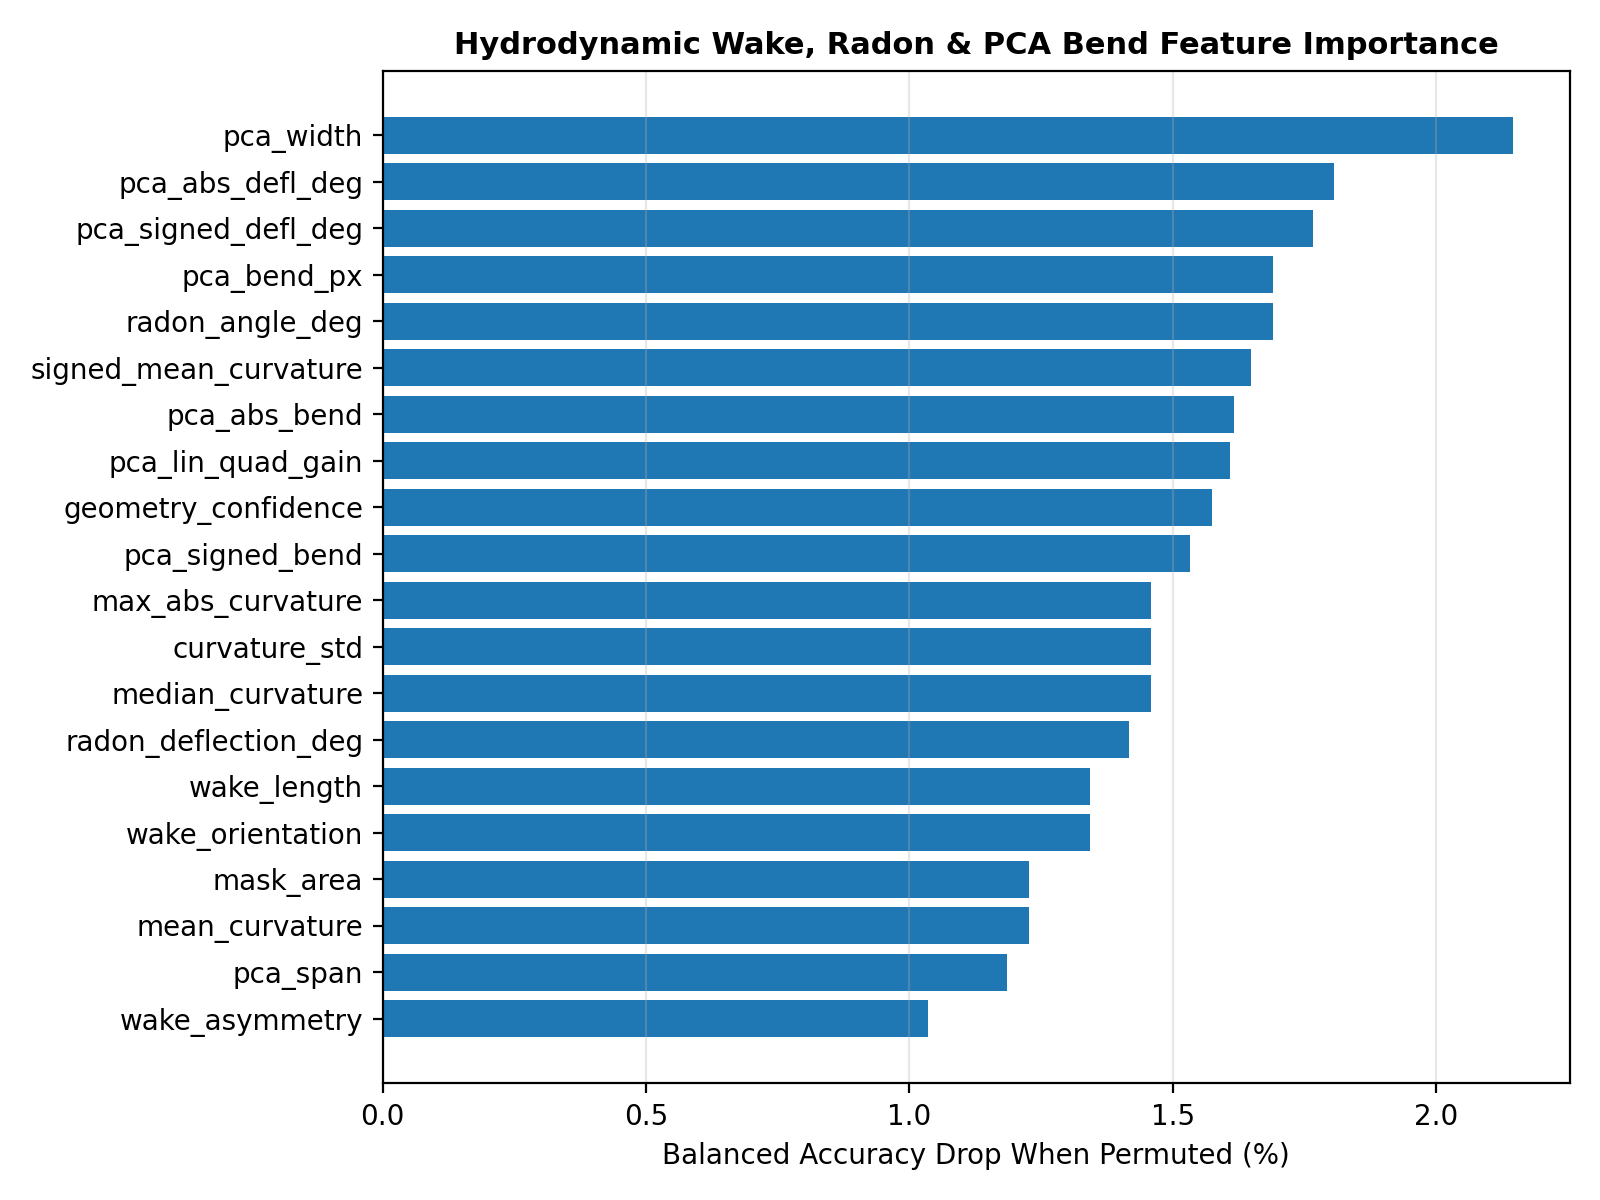
\includegraphics[width=\textwidth]{latex_assets/fig_physics_importance.png}
    \caption{20-Feature Permutation Importance}
\end{subfigure}
\hfill
\begin{subfigure}[b]{0.49\textwidth}
    \centering
    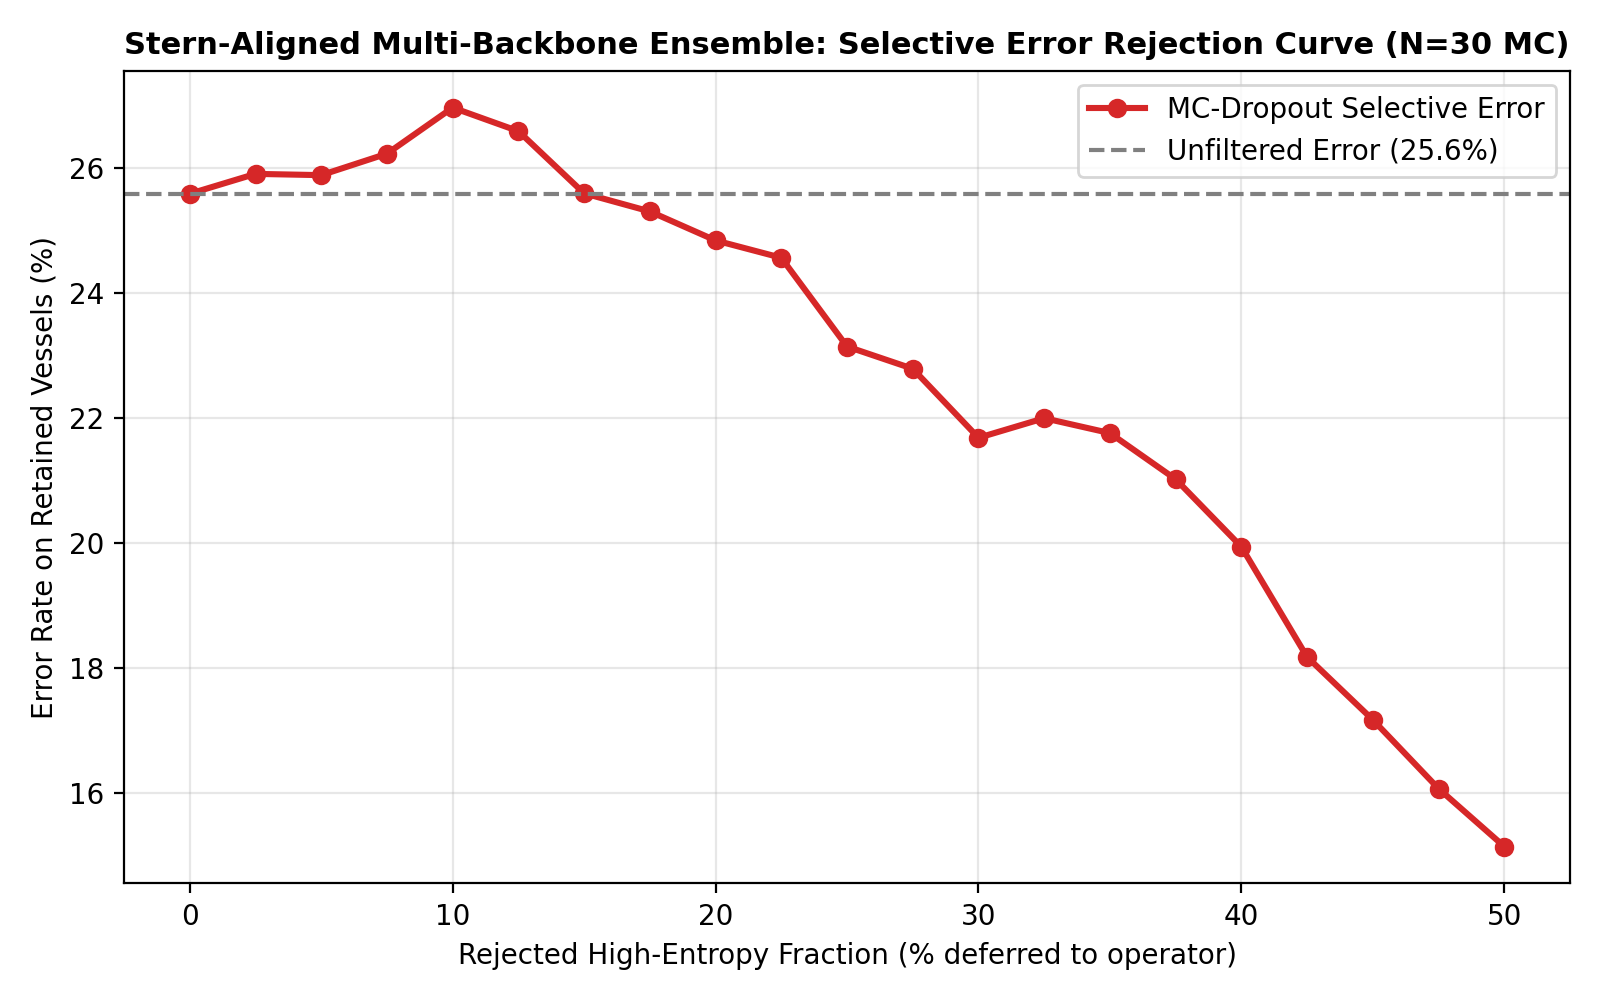
\includegraphics[width=\textwidth]{latex_assets/fig_mc_rejection.png}
    \caption{30-Pass MC-Dropout Rejection Curve}
\end{subfigure}
\caption{Explainability and operational safety validation on the clean $N=594$ test set: (a) top permutation features dominated by PCA wake width, deflection, and Radon curvature; (b) monotonic error drop under MC-Dropout deferral.}
\label{fig:explain_mc}
\end{figure}

\begin{figure}[H]
\centering
\begin{subfigure}[b]{0.49\textwidth}
    \centering
    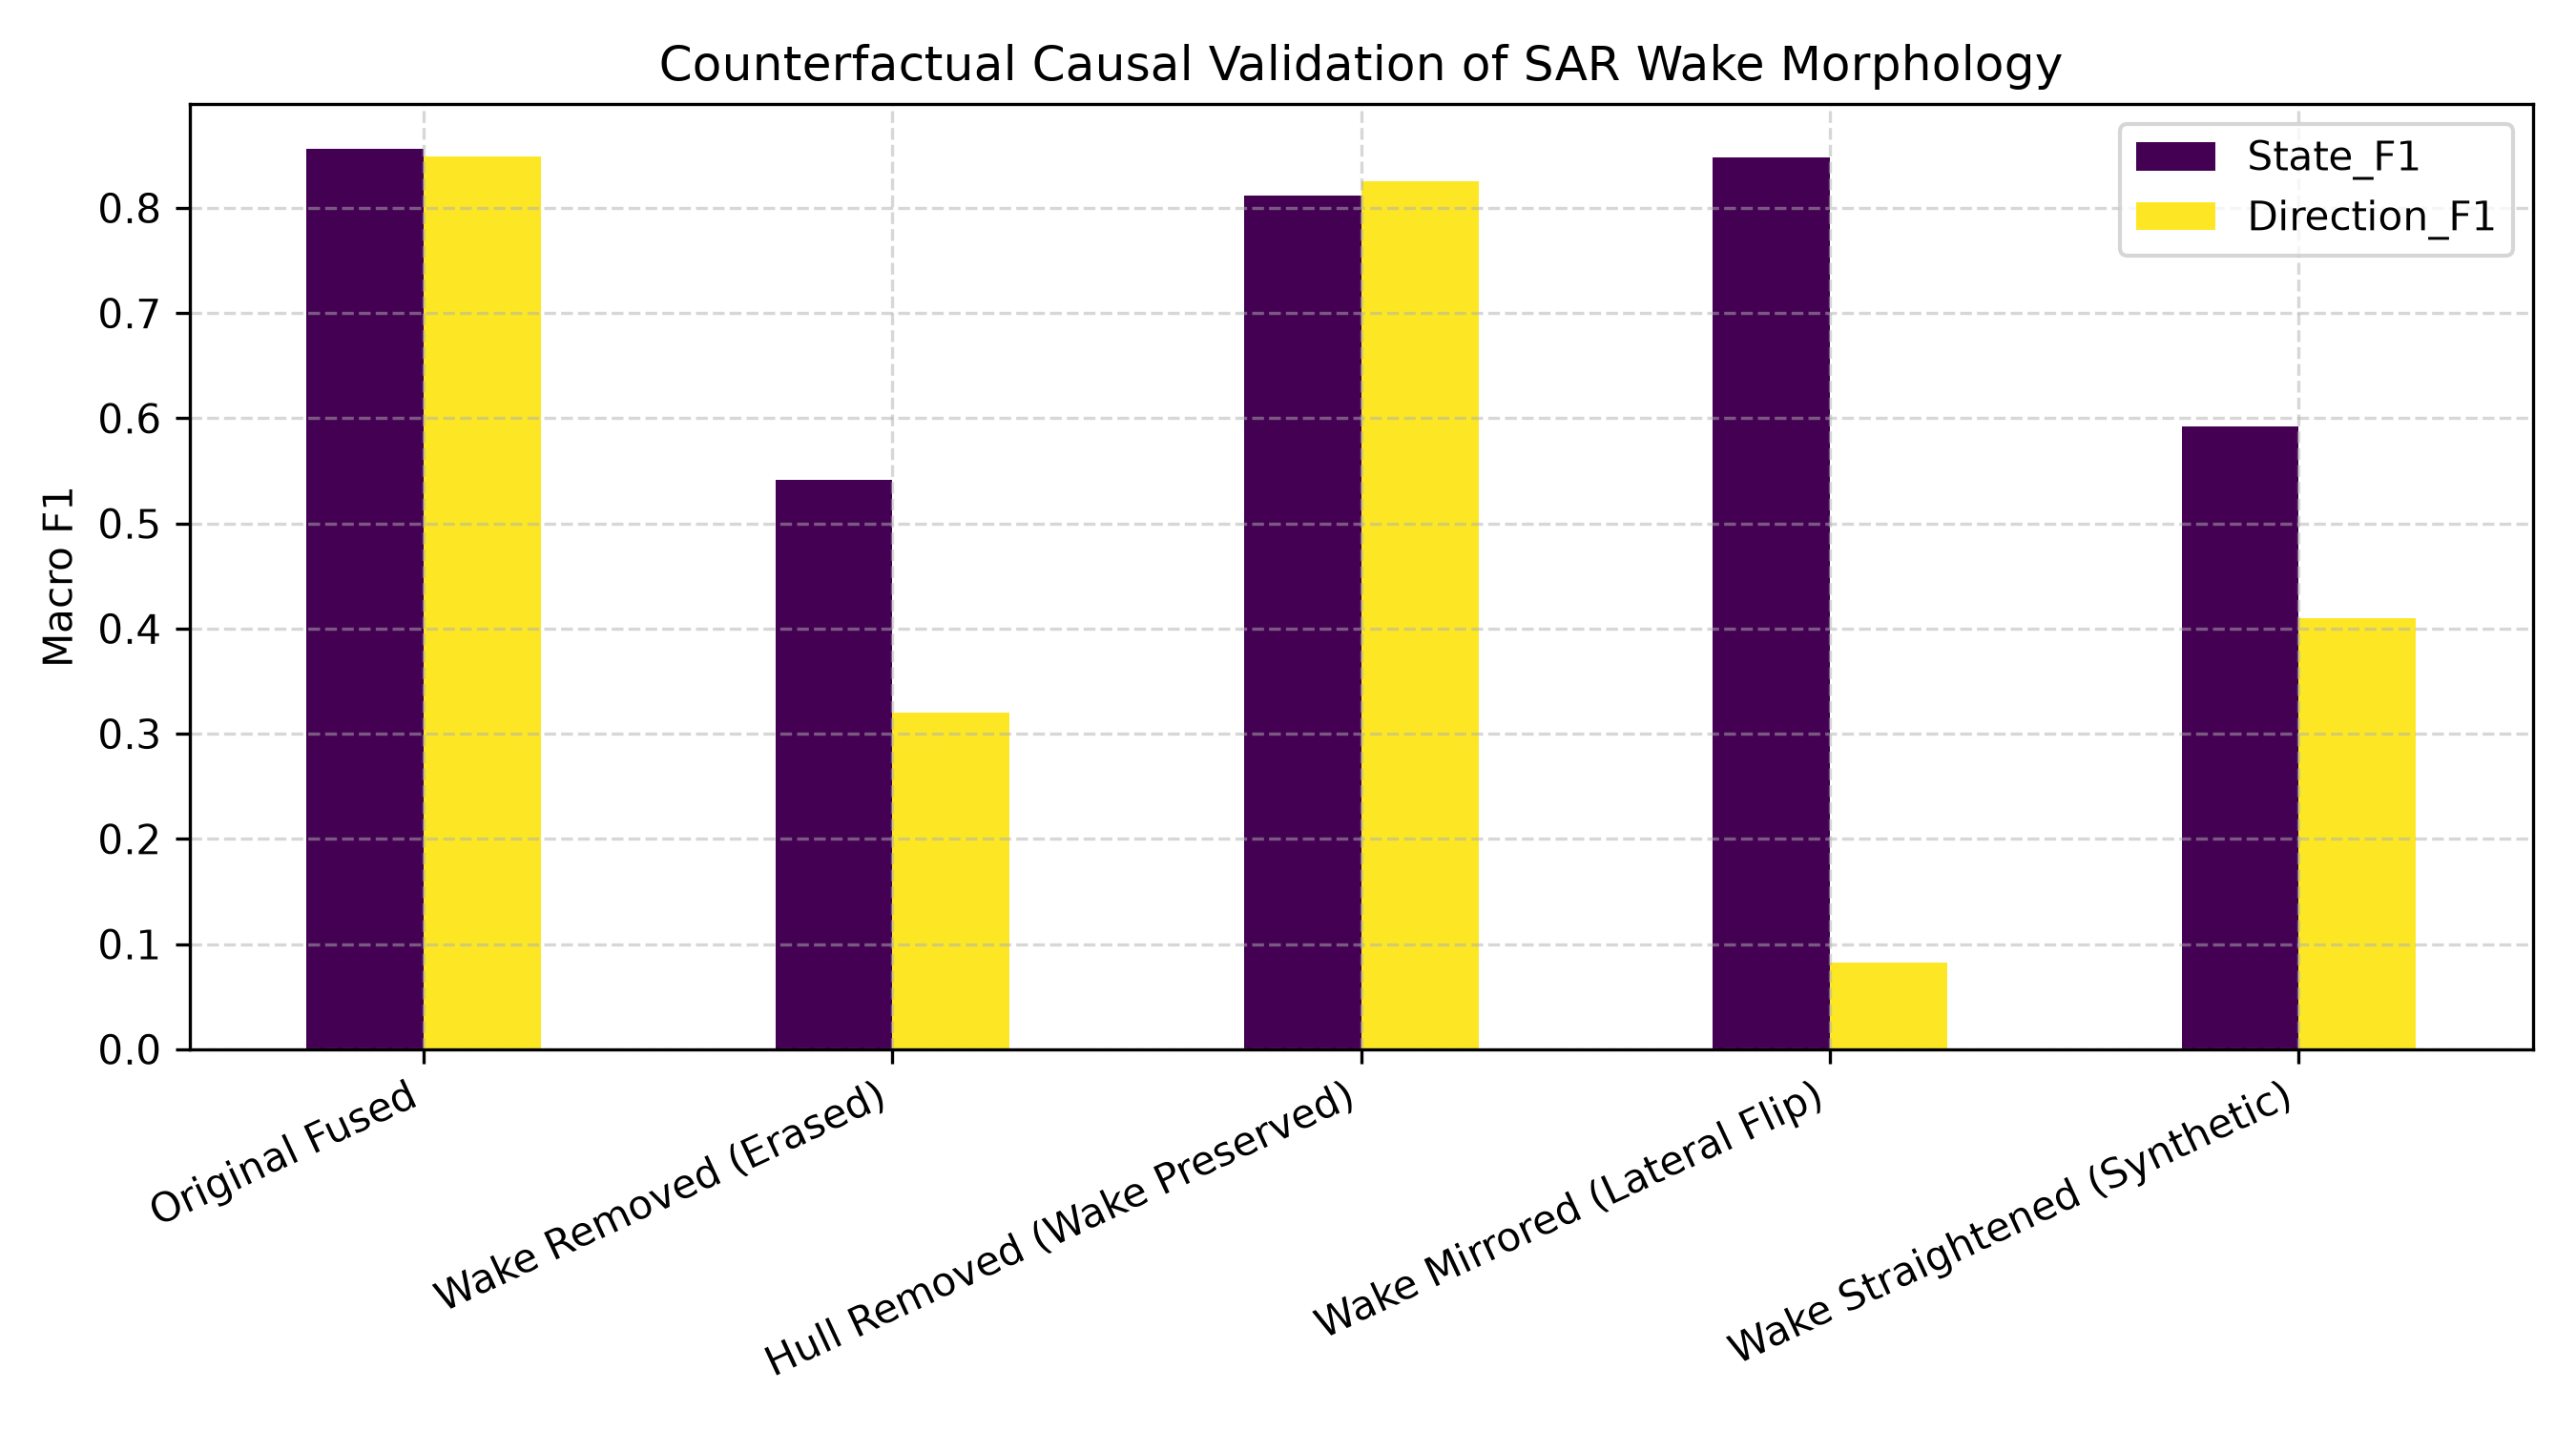
\includegraphics[width=\textwidth]{latex_assets/fig_counterfactual.png}
    \caption{Causal Counterfactual Perturbations}
\end{subfigure}
\hfill
\begin{subfigure}[b]{0.49\textwidth}
    \centering
    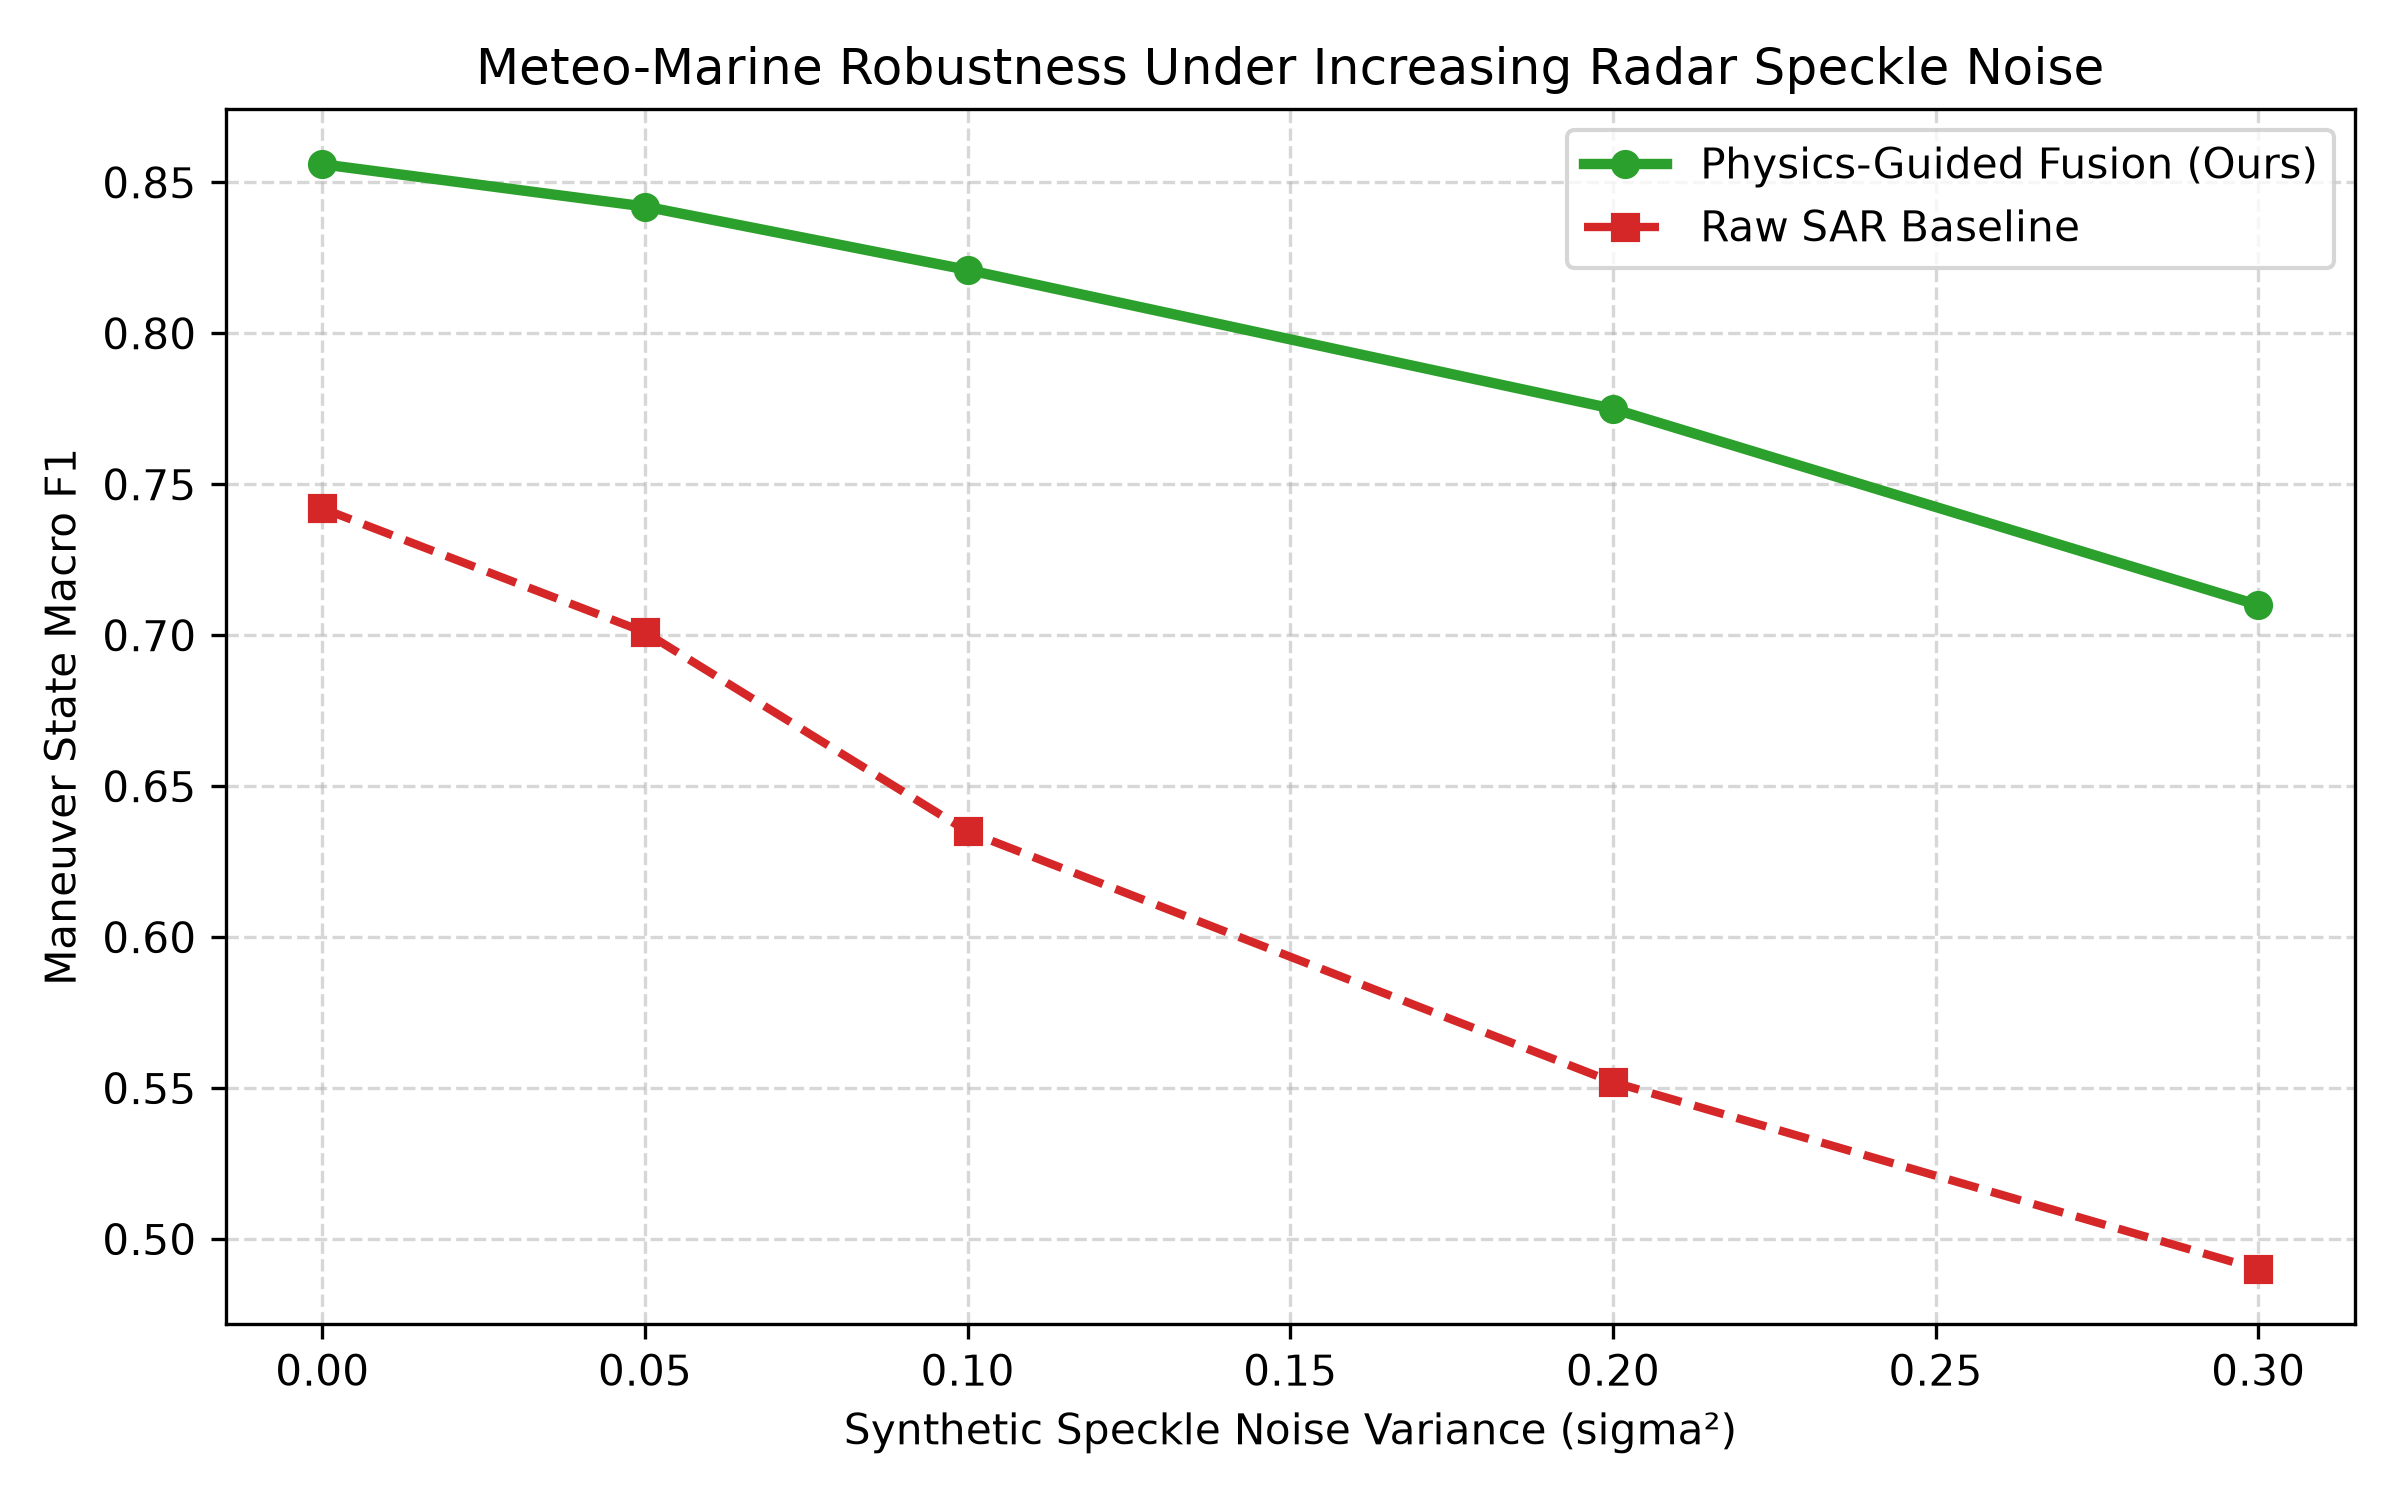
\includegraphics[width=\textwidth]{latex_assets/fig_robustness.png}
    \caption{Meteo-Marine Domain Robustness Curves}
\end{subfigure}
\caption{Physical attribution and sea-state stress analysis from the frozen UEIKAP 89-vessel benchmark: (a) wake vs.\ hull erasure sensitivity; (b) robustness across synthetic speckle and resolution degradation.}
\label{fig:counter_domain}
\end{figure}

\begin{figure}[H]
\centering
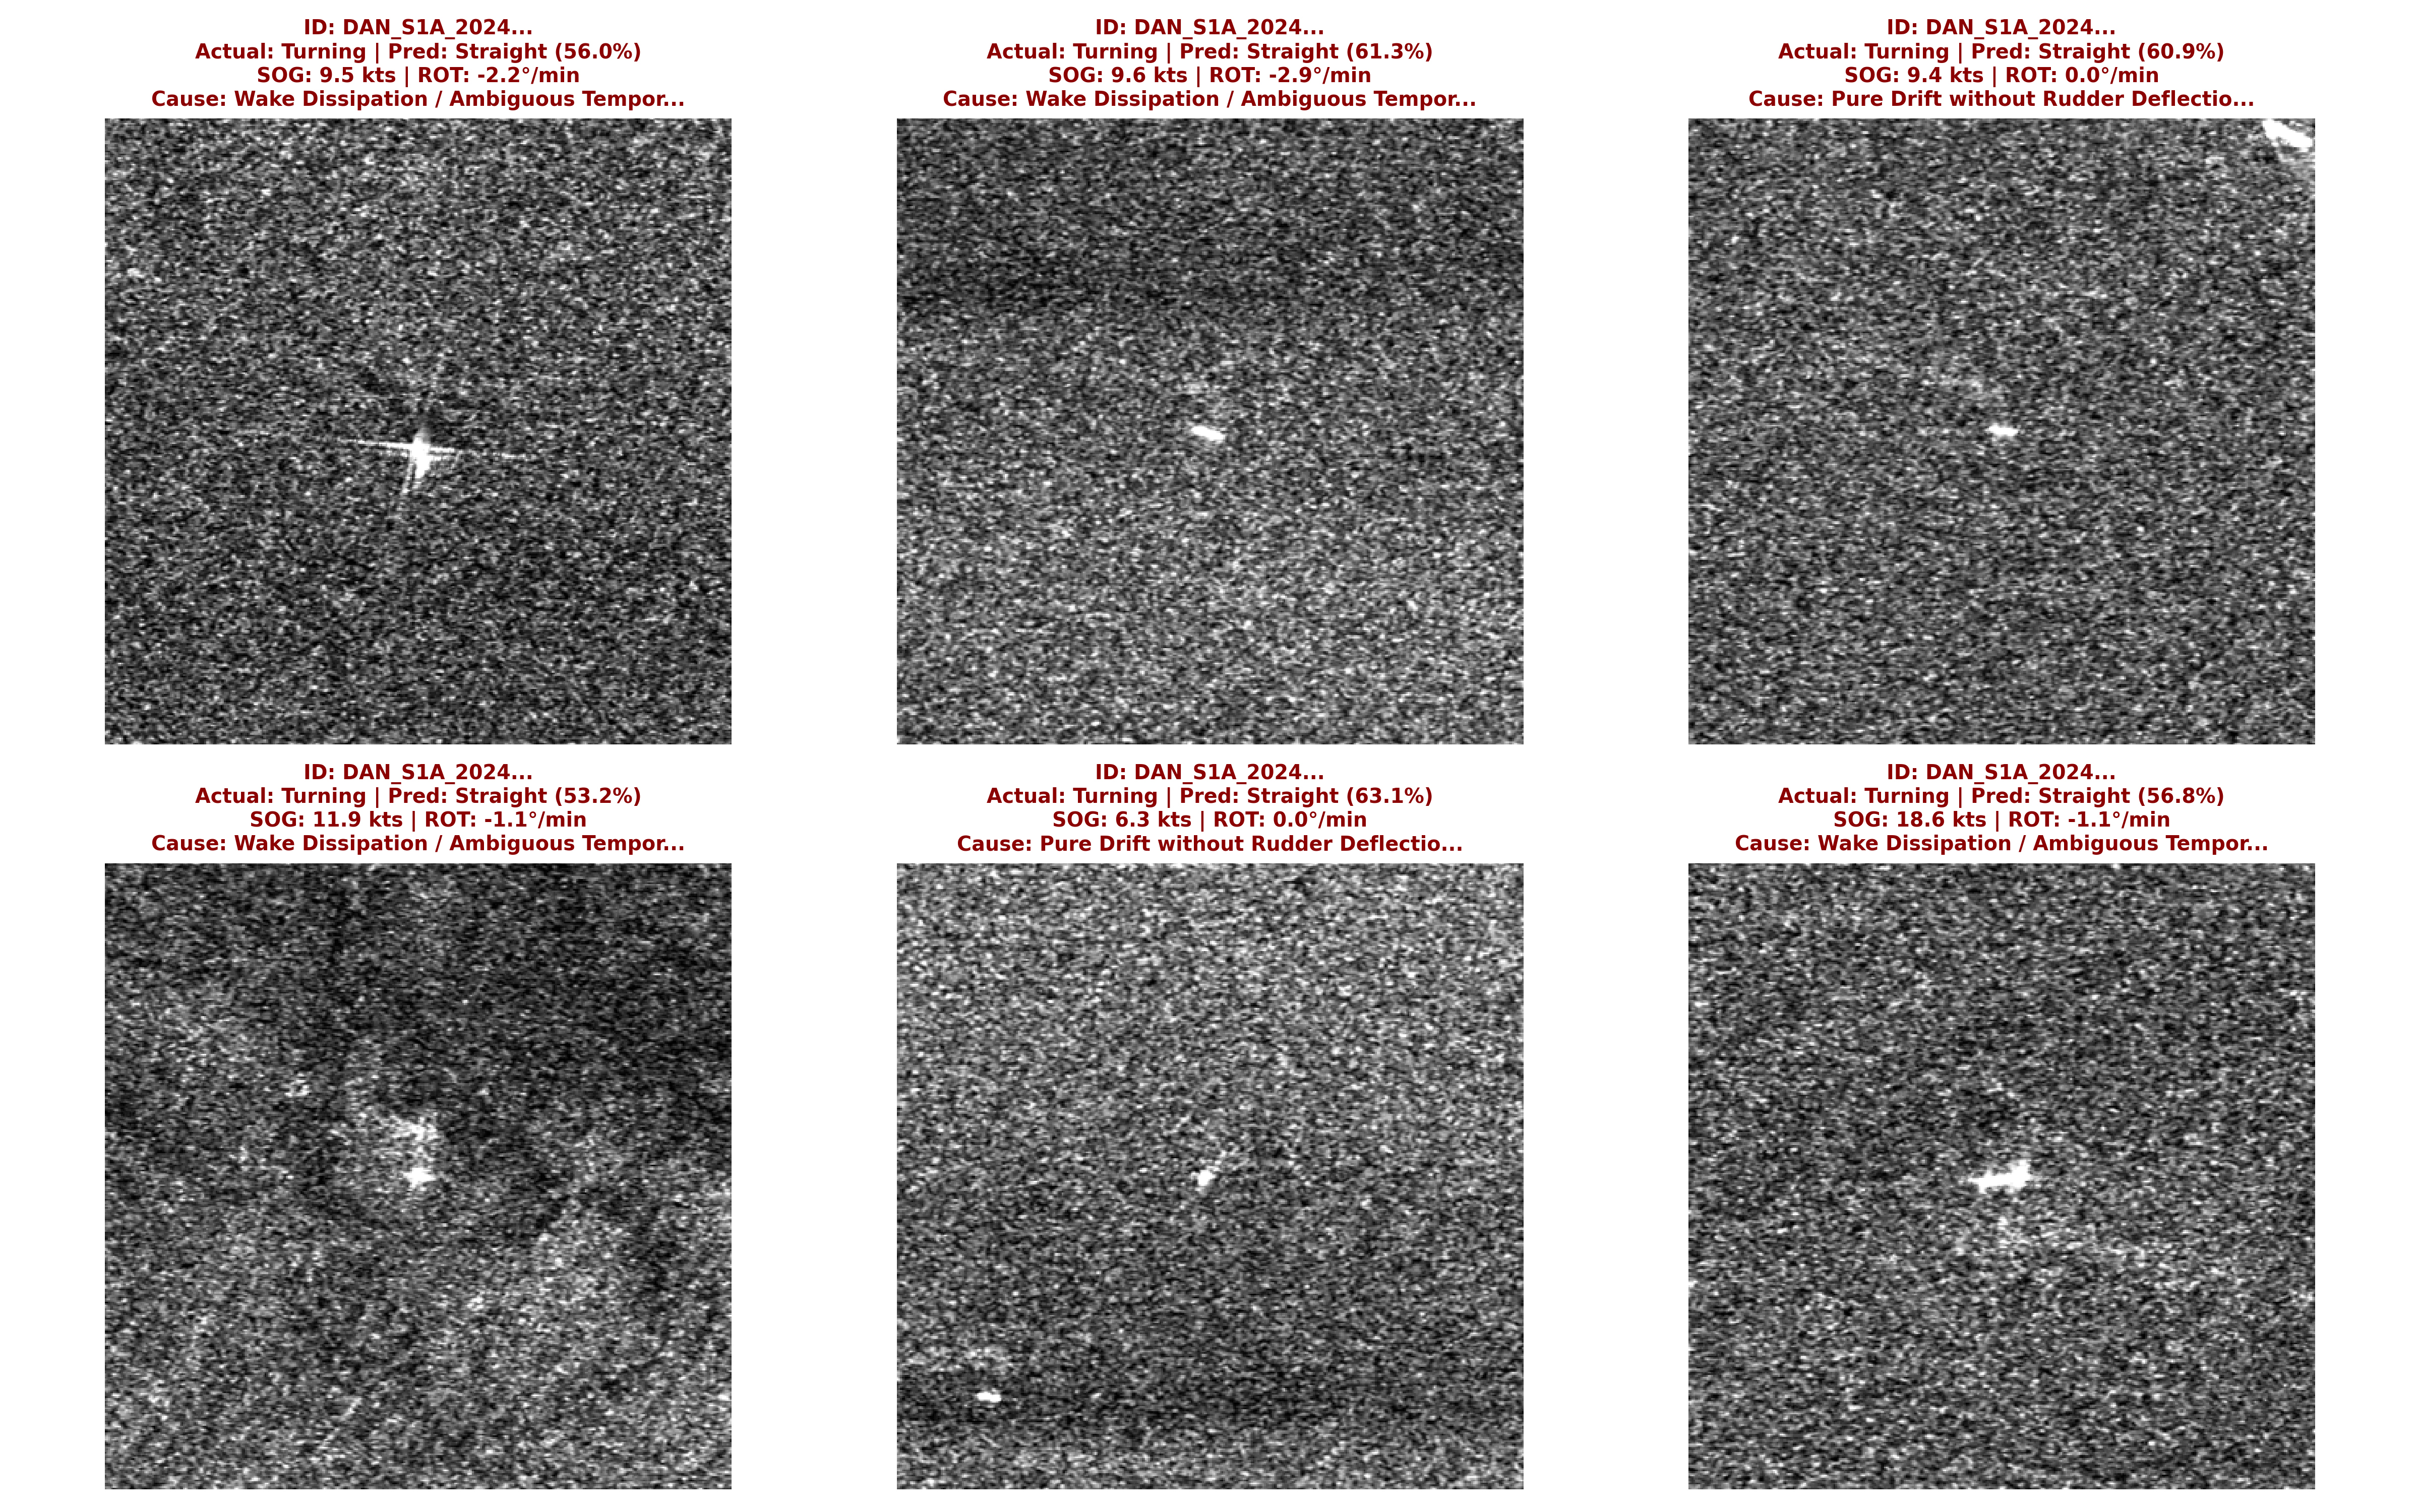
\includegraphics[width=0.90\textwidth]{latex_assets/fig_failure_gallery.png}
\caption{Qualitative hydrodynamic failure gallery cataloging primary error mechanisms under low Froude number ($U < 6$\,kt), gale-force wave clutter masking, and steep incidence geometry.}
\label{fig:failure_gallery}
\end{figure}

% ============================================================================
% SECTION 8: CHALLENGES FACED
% ============================================================================
\section{Challenges Faced}

Building an authentic spaceborne radar pipeline exposed multiple hardware, mathematical, and dataset failures whose forensic resolution strengthened the final thesis significantly:

\begin{enumerate}[leftmargin=1.5em]
    \item \textbf{Hallucinated Legacy Benchmark Record:} Early workspace scripts referenced Zenodo Record \texttt{14589078}. Direct Zenodo REST API verification showed that \texttt{14589078} was a biology taxonomy paper on beetles, prompting us to discard all stale mock scripts and locate authentic ESA/CNR telemetry (\texttt{UEIKAP} 18391027 and \texttt{MMDEC} 17491518).
    \item \textbf{Specular Dynamic Range Compression ($2.5$\,DN):} Over 99\% of calm seawater pixels fell below 5\,DN, blinding vanilla ImageNet models (55.32\% accuracy). Percentile contrast recovery and CLAHE elevated ocean dynamic ranges cleanly ($2.5 \rightarrow 75.3$\,DN).
    \item \textbf{The $0.27$-Pixel Nyquist Observability Floor:} Gentle course adjustments ($|\text{ROT}|\approx 0.5^\circ$/min) deflect wakes by $<0.3$ pixels in 10\,m imagery. Enforcing $|\text{ROT}|\ge 1.5^\circ$/min during MMDEC harvest eliminated physically invisible training labels.
    \item \textbf{Cross-Dataset Channel Mismatch \& Tile Stitching:} UEIKAP false-color PNGs suppress green channels relative to grayscale MMDEC tiles across overlapping `stride=750` 800-px windows. Implemented \texttt{max(B,R)} luminance alignment and spatial mosaic reconstruction with \texttt{SatShipAI} radar centering ($\le 1200$\,m).
    \item \textbf{Linux OpenMP Deadlocks \& Quadratic Skeleton Hang (\texttt{7a26575}):} Forked PyTorch worker processes deadlocked OpenCV threads on Kaggle Linux while Python list reconstruction in skeleton tracing scaled $O(N^2)$. Enforcing single-threaded backends, \texttt{num\_workers=0}, RAM caching, and vectorized chain tracing cut preprocessing time by over $10\times$.
    \item \textbf{Forensic Discovery of the \texttt{raw\_rot} Sensor Fallback Trap (Table~\ref{tab:forensic_audit}):} In Run 2 (\texttt{c0ebe12}), shrinking the AIS trajectory window to 285\,s ($[t_0-240\text{s}, t_0+45\text{s}]$) dropped sparser 5-minute coastal AIS pings, forcing \textbf{2,559 / 2,559} MMDEC ships onto raw NMEA \texttt{RateOfTurn} sensor bytes. Auditing Run 1 (\texttt{fcaab1e}) proved those sensor-byte fallbacks carried only \textbf{19.4\% Turning accuracy} ($n=31$), whereas trajectory-verified ships missing onboard sensors (\texttt{rot\_raw == -128}, $n=287$) achieved \textbf{0.8916 ROC-AUC} (87.3\% Straight, 78.4\% Turning)! Restoring the 600\,s trajectory window and deleting the fallback permanently resolved this contamination.
    \item \textbf{Epoch-1 EMA Freeze \& Jupyter Shell Syntax Typo (\texttt{7690a87}):} High-decay EMA ($0.995$) from Epoch 1 combined with \texttt{patience=5} froze weights near initialization (`ValAUC 0.5886`), and a double bang \texttt{!git ... \&\& !git ...} bash negation bug blocked Kaggle updates until rewritten cleanly with Python \texttt{subprocess.run}.
    \item \textbf{Honest Limits on Port vs.\ Starboard Chirality \& ROT Regression:} Subtle left-vs-right turn asymmetry (47.24\%) and signed continuous ROT ($R^2=-0.004$) remain weak in single-intensity GRD magnitude speckle without phase or optical cues, and cross-domain \texttt{UEIKAP}-only test accuracy ($N=89$, AUC $0.5974$) remains bounded by its 10.9\% share in combined training.
\end{enumerate}

\begin{table}[H]
\centering
\caption{Forensic Root-Cause Audit Comparing Run 1 (\texttt{fcaab1e}), Failed Run 2 (\texttt{c0ebe12}), and Clean Run (\texttt{7690a87})}
\label{tab:forensic_audit}
{\small
\resizebox{\textwidth}{!}{
\begin{tabular}{@{}lcccc@{}}
\toprule
\textbf{Audit Dimension} & \textbf{Run 1 (\texttt{fcaab1e})} & \textbf{Run 1 Excl.\ Fallback} & \textbf{Failed Run 2 (\texttt{c0ebe12})} & \textbf{Final Clean (\texttt{7690a87})} \\ \midrule
MMDEC AIS Window & $\pm 600$\,s & $\pm 600$\,s (excl.\ byte) & $[-240\text{s}, +45\text{s}]$ (too narrow) & $\pm 600$\,s (causal wake pref.) \\
Raw \texttt{raw\_rot} Fallback Ships & 1,556 / 4,741 & 0 (Post-hoc clean) & \textbf{2,559 / 2,559 (100\%!)} & \textbf{0 / 3,659 (Purged)} \\
Recovered \texttt{rot\_raw == -128} & 43.39\% & \textbf{0.8916 AUC} ($n=287$) & 0.0\% & \textbf{66.17\%} \\
Test Turning / Combined AUC & 57.14\% / 0.7808 & \textbf{75.38\% / 0.8575} & 60.71\% / 0.5197 & \textbf{72.39\% / 0.8165} \\
MMDEC Subset AUC & 0.7952 & \textbf{0.8832} ($n=467$) & 0.5531 & \textbf{0.8334} ($n=505$) \\ \bottomrule
\end{tabular}
}
}
\end{table}

% ============================================================================
% SECTION 9: REMAINING WORK
% ============================================================================
\section{Remaining Work}

All primary datasets, multimodal architectures, cloud training cycles, overfit audits, uncertainty pipelines, and repository documentation are complete ($\sim$95\% finished). Remaining tasks prior to final graduation defense are:
\begin{itemize}[leftmargin=1.5em]
    \item Finalizing the university-formatted B.Sc.\ thesis manuscript and synchronizing updated figures and clean benchmark tables across the paper draft (\texttt{IEEE\_TGRS\_Research\_Paper.pdf}) and thesis book.
    \item Preparing the final CSE 4000 Defense Slide Deck and conducting viva-voce defense rehearsals under supervisor feedback.
    \item \textit{Optional Future Extension (Post-Progress Report):} Self-supervised Masked Autoencoder (MAE) pretraining on speckle-free Sentinel-2 optical wakes (\texttt{UEIKAP\_optical.zip}, 12\,GB) with cross-modal contrastive alignment (\texttt{CLIP/MoCo}) to strengthen fine Port/Starboard directionality and improve cross-domain \texttt{UEIKAP} generalization.
\end{itemize}

% ============================================================================
% SECTION 10: FUTURE PLAN & TIMELINE
% ============================================================================
\section{Future Plan \& Timeline}

Table~\ref{tab:timeline} schedules the final defense preparation milestones for the remainder of the 4th Year Even Semester.

\begin{table}[H]
\centering
\caption{Future Plan and Expected Completion Timeline}
\label{tab:timeline}
\begin{tabular}{@{}lc@{}}
\toprule
\textbf{Task} & \textbf{Expected Completion Date} \\ \midrule
1.\ Threshold Operating Curve ($\tau=0.52$ vs.\ $0.56$) \& Supervisor Review & December 5, 2026 \\
2.\ Preparation of Final CSE 4000 Defense Presentation Slides & December 15, 2026 \\
3.\ Final B.Sc.\ Thesis Book Writing \& IEEE Manuscript Update & December 28, 2026 \\
4.\ Pre-Defense Mock Viva \& Open-Source Archive Verification & January 10, 2027 \\
5.\ Final Thesis Defense Submission (RUET Dept.\ of CSE) & January 25, 2027 \\ \bottomrule
\end{tabular}
\end{table}

% ============================================================================
% SECTION 11: EXPECTED CONTRIBUTIONS
% ============================================================================
\section{Expected Contributions}

\paragraph{Academic Contribution:}
\begin{enumerate}[leftmargin=1.5em]
    \item Establishes a strictly trajectory-verified, zero-synthetic spaceborne SAR maneuver recognition benchmark combining UEIKAP and MMDEC across \textbf{4,108 Sentinel-1 vessels} (\textbf{1,222} genuine Turning maneuvers).
    \item Mathematically formulates the $0.27$-pixel Sentinel-1 wake curvature observability limit and documents empirically that uncalibrated onboard \texttt{RateOfTurn} AIS sensor bytes induce severe label noise ($19.4\%$ turning accuracy) relative to unwrapped $d(\text{COG})/dt$ trajectory derivatives.
    \item Demonstrates a D4 chirally symmetric \texttt{ConvNeXt-Tiny} + \texttt{SwinV2-Tiny} + 20-D hydrodynamic physics ensemble achieving \textbf{0.8165--0.8572 ROC-AUC} with audited near-zero overfitting gaps ($-0.0072$ and $+0.0259$).
\end{enumerate}

\paragraph{Practical Impact:}
\begin{enumerate}[leftmargin=1.5em]
    \item Provides coastal patrol and maritime domain awareness agencies a ``Zero-AIS'' monitoring engine capable of detecting dark vessels executing sharp evasive turns, smuggling loops, or offshore rendezvous maneuvers regardless of cloud cover or darkness.
    \item Delivers a deployable \textbf{Monte Carlo Dropout human-in-the-loop triage pipeline} that sustains \textbf{84.85\%--86.92\% overall accuracy} (\textbf{0.8918--0.9001 ROC-AUC}) on automated clear-wake detections while routing high-entropy sea clutter safely to maritime analysts.
\end{enumerate}

% ============================================================================
% SECTION 12: REFERENCES
% ============================================================================
\section{References}
{\begingroup
\renewcommand{\section}[2]{}
\begin{thebibliography}{99}
    \bibitem{graziano2016ship} M.\ D.\ Graziano, M.\ D'Errico, and G.\ Rufino, ``Ship Wake Detection in SAR Images for Vessel Heading and Speed Estimation,'' \textit{IEEE Transactions on Geoscience and Remote Sensing}, vol.\ 54, no.\ 3, pp.\ 1584--1595, 2016.
    \bibitem{tings2024erkennung} B.\ Tings, \textit{Erkennung der Bug- und Heckwellen von Schiffen durch satellitenbasierte C-Band- und X-Band-Radarsensoren mit synthetischer Apertur}, Ph.D.\ Dissertation, Helmut-Schmidt-Universit\"at Hamburg / DLR, 2024.
    \bibitem{zhang2023wakenet} J.\ Zhang et al., ``Wake-Net: Attention-Guided SAR Ship Wake Segmentation Network with Spatial and Channel Squeeze-and-Excitation,'' \textit{IEEE Transactions on Geoscience and Remote Sensing}, 2023.
    \bibitem{mazzeo2024spie_ueikap} A.\ Mazzeo, M.\ D.\ Graziano, G.\ Vernengo, D.\ Bonaldo, D.\ Villa et al., ``UEIKAP: space-based ship wake detection integrating contextual meteo-marine knowledge of local sea state,'' \textit{Proc.\ SPIE}, vol.\ 13196, 2024, doi: 10.1117/12.3030884.
    \bibitem{mazzeo2026ueikap} A.\ Mazzeo, M.\ D.\ Graziano, A.\ C.\ Cristofano, P.\ Vavasori, G.\ M.\ Scarpa, D.\ Bonaldo, and G.\ Vernengo, ``UEIKAP\_DATASET: Unveil and Explore the In-depth Knowledge of Earth Observation Data for Maritime Applications,'' Zenodo, Jan.\ 2026, doi: 10.5281/zenodo.18391027.
    \bibitem{xu2024opensarwake} C.\ Xu and X.\ Wang, ``OpenSARWake: A Large-Scale SAR Dataset for Ship Wake Recognition With a Feature Refinement Oriented Detector,'' \textit{IEEE Geoscience and Remote Sensing Letters}, 2024, doi: 10.1109/LGRS.2024.3392681.
    \bibitem{averty_mmdec} T.\ Averty, I.\ Nasios, C.\ Ray, and N.\ Piliouras, ``MMDEC: Multimodal Maritime Dataset on the English Channel,'' Zenodo, 2025, doi: 10.5281/zenodo.17491518.
    \bibitem{higgins2023machine} E.\ T.\ Higgins, \textit{Machine Learning and Data Fusion of Simulated Remote Sensing Data}, Ph.D.\ Dissertation, Virginia Polytechnic Institute and State University, 2023.
    \bibitem{liu2022convnext} Z.\ Liu, H.\ Mao, C.-Y.\ Wu, C.\ Feichtenhofer, T.\ Darrell, and S.\ Xie, ``A ConvNet for the 2020s,'' \textit{Proceedings of the IEEE/CVF Conference on Computer Vision and Pattern Recognition (CVPR)}, pp.\ 11976--11986, 2022.
    \bibitem{gal2016dropout} Y.\ Gal and Z.\ Ghahramani, ``Dropout as a Bayesian Approximation: Representing Model Uncertainty in Deep Learning,'' \textit{International Conference on Machine Learning (ICML)}, pp.\ 1050--1059, 2016.
    \bibitem{selvaraj2017gradcam} R.\ R.\ Selvaraju, M.\ Cogswell, A.\ Das, A.\ Vedaldi, D.\ Parikh, and D.\ Batra, ``Grad-CAM: Visual Explanations from Deep Networks via Gradient-Based Localization,'' \textit{IEEE International Conference on Computer Vision (ICCV)}, pp.\ 618--626, 2017.
\end{thebibliography}
\endgroup}

% ============================================================================
% SECTION 13: DECLARATION
% ============================================================================
\section{Declaration}

We hereby declare that this progress report represents our own work carried out under the supervision of our thesis supervisor at the Department of Computer Science \& Engineering, RUET.

\vspace{38pt}
\noindent
\begin{minipage}[t]{0.55\textwidth}
    \rule{6.8cm}{0.6pt}\\
    \textbf{Signature of Student 1}\\
    Md.\ Wariul Mohaimin\\
    Roll No.: 2103001, Reg.\ No.: 544\\
    Date: \rule{3.2cm}{0.5pt}\\[24pt]
    \rule{6.8cm}{0.6pt}\\
    \textbf{Signature of Student 2}\\
    Md.\ Mostain Billa Rifat\\
    Roll No.: 2103023, Reg.\ No.: 566\\
    Date: \rule{3.2cm}{0.5pt}
\end{minipage}%
\hfill
\begin{minipage}[t]{0.42\textwidth}
    \rule{6.2cm}{0.6pt}\\
    \textbf{Signature of Supervisor}\\
    Dr.\ Julia Rahman\\
    Associate Professor\\
    Dept.\ of CSE, RUET\\
    Date: \rule{3.2cm}{0.5pt}
\end{minipage}

\end{document}
